\documentclass[runningheads]{llncs}

% ---------------------------------------------------------------
% Include basic ECCV package
 
% TODO REVIEW: Insert your submission number below by replacing '*****'
% TODO FINAL: Comment out the following line for the camera-ready version
\usepackage[review,year=2024,ID=8436]{eccv}
% TODO FINAL: Un-comment the following line for the camera-ready version
%\usepackage{eccv}

% OPTIONAL: Un-comment the following line for a version which is easier to read
% on small portrait-orientation screens (e.g., mobile phones, or beside other windows)
%\usepackage[mobile]{eccv}

\usepackage{multirow} % Required for multirows
\usepackage{colortbl}
\usepackage{array}
\usepackage{wrapfig}

% ---------------------------------------------------------------
% Other packages

% Commonly used abbreviations (\eg, \ie, \etc, \cf, \etal, etc.)
\usepackage{eccvabbrv}

% Include other packages here, before hyperref.
\usepackage{graphicx}
\usepackage{booktabs}

% The "axessiblity" package can be found at: https://ctan.org/pkg/axessibility?lang=en
\usepackage[accsupp]{axessibility}  % Improves PDF readability for those with disabilities.


% ---------------------------------------------------------------
% Hyperref package

% It is strongly recommended to use hyperref, especially for the review version.
% Please disable hyperref *only* if you encounter grave issues.
% hyperref with option pagebackref eases the reviewers' job, but should be disabled for the final version.
%
% If you comment hyperref and then uncomment it, you should delete
% main.aux before re-running LaTeX.
% (Or just hit 'q' on the first LaTeX run, let it finish, and you
%  should be clear).

% TODO FINAL: Comment out the following line for the camera-ready version
\usepackage[pagebackref,breaklinks,colorlinks,citecolor=eccvblue]{hyperref}
% TODO FINAL: Un-comment the following line for the camera-ready version
%\usepackage{hyperref}

% Support for ORCID icon
\usepackage{orcidlink}


\begin{document}

% ---------------------------------------------------------------
% TODO REVIEW: Replace with your title
\title{Skeleton2vec: A Self-supervised Learning Framework with Contextualized Target Representations for Skeleton Sequence} 

% TODO REVIEW: If the paper title is too long for the running head, you can set
% an abbreviated paper title here. If not, comment out.
\titlerunning{Skeleton2vec}

% TODO FINAL: Replace with your author list. 
% Include the authors' OCRID for the camera-ready version, if at all possible.
\author{First Author\inst{1}\orcidlink{0000-1111-2222-3333} \and
Second Author\inst{2,3}\orcidlink{1111-2222-3333-4444} \and
Third Author\inst{3}\orcidlink{2222--3333-4444-5555}}

% TODO FINAL: Replace with an abbreviated list of authors.
\authorrunning{F.~Author et al.}
% First names are abbreviated in the running head.
% If there are more than two authors, 'et al.' is used.

% TODO FINAL: Replace with your institution list.
\institute{Princeton University, Princeton NJ 08544, USA \and
Springer Heidelberg, Tiergartenstr.~17, 69121 Heidelberg, Germany
\email{lncs@springer.com}\\
\url{http://www.springer.com/gp/computer-science/lncs} \and
ABC Institute, Rupert-Karls-University Heidelberg, Heidelberg, Germany\\
\email{\{abc,lncs\}@uni-heidelberg.de}}

\maketitle

\begin{abstract}
Self-supervised pre-training paradigms have been extensively explored in the field of
skeleton-based action recognition. In particular, methods based on
\textbf{masked prediction} have pushed the performance of pre-training to a new height.
However, these methods take low-level features, such as raw joint coordinates or
temporal motion, as prediction targets for the masked regions, which is suboptimal.
In this paper, we show that using high-level contextualized features as prediction
targets can achieve superior performance. Specifically, we propose \textbf{Skeleton2vec},
a simple and efficient self-supervised 3D action representation learning framework,
which utilizes a transformer-based teacher encoder taking unmasked training samples as
input to create \textbf{latent contextualized representations} as prediction targets.
Benefiting from the self-attention mechanism, the latent representations generated by
the teacher encoder can incorporate the global context of the entire training samples,
leading to a richer training task.
% can interact with the whole skeleton sequence, thereby possessing
% stronger spatio-temporal contextual associations and richer semantics.
Additionally, considering the high temporal correlations in skeleton sequences, we propose a
\textbf{Motion-Aware Multi-Tube masking strategy} which divides the skeleton sequence into
multiple tubes and performs persistent masking within each tube based on motion priors,
thus forcing the model to build long-range spatio-temporal connections and focus on
action-semantic richer regions. Extensive experiments on NTU-60, NTU-120, and PKU-MMD
datasets demonstrate that our proposed Skeleton2vec outperforms previous methods and
achieves state-of-the-art results.
The code will be made available after the paper is accepted for publication.
\keywords{Self-supervised 3D action recognition \and Masking prediction}
\end{abstract}    
\section{Introduction}
\label{sec:intro}

\begin{figure}[tb]
	\centering
	\begin{subfigure}{0.3\linewidth}
		\centering
		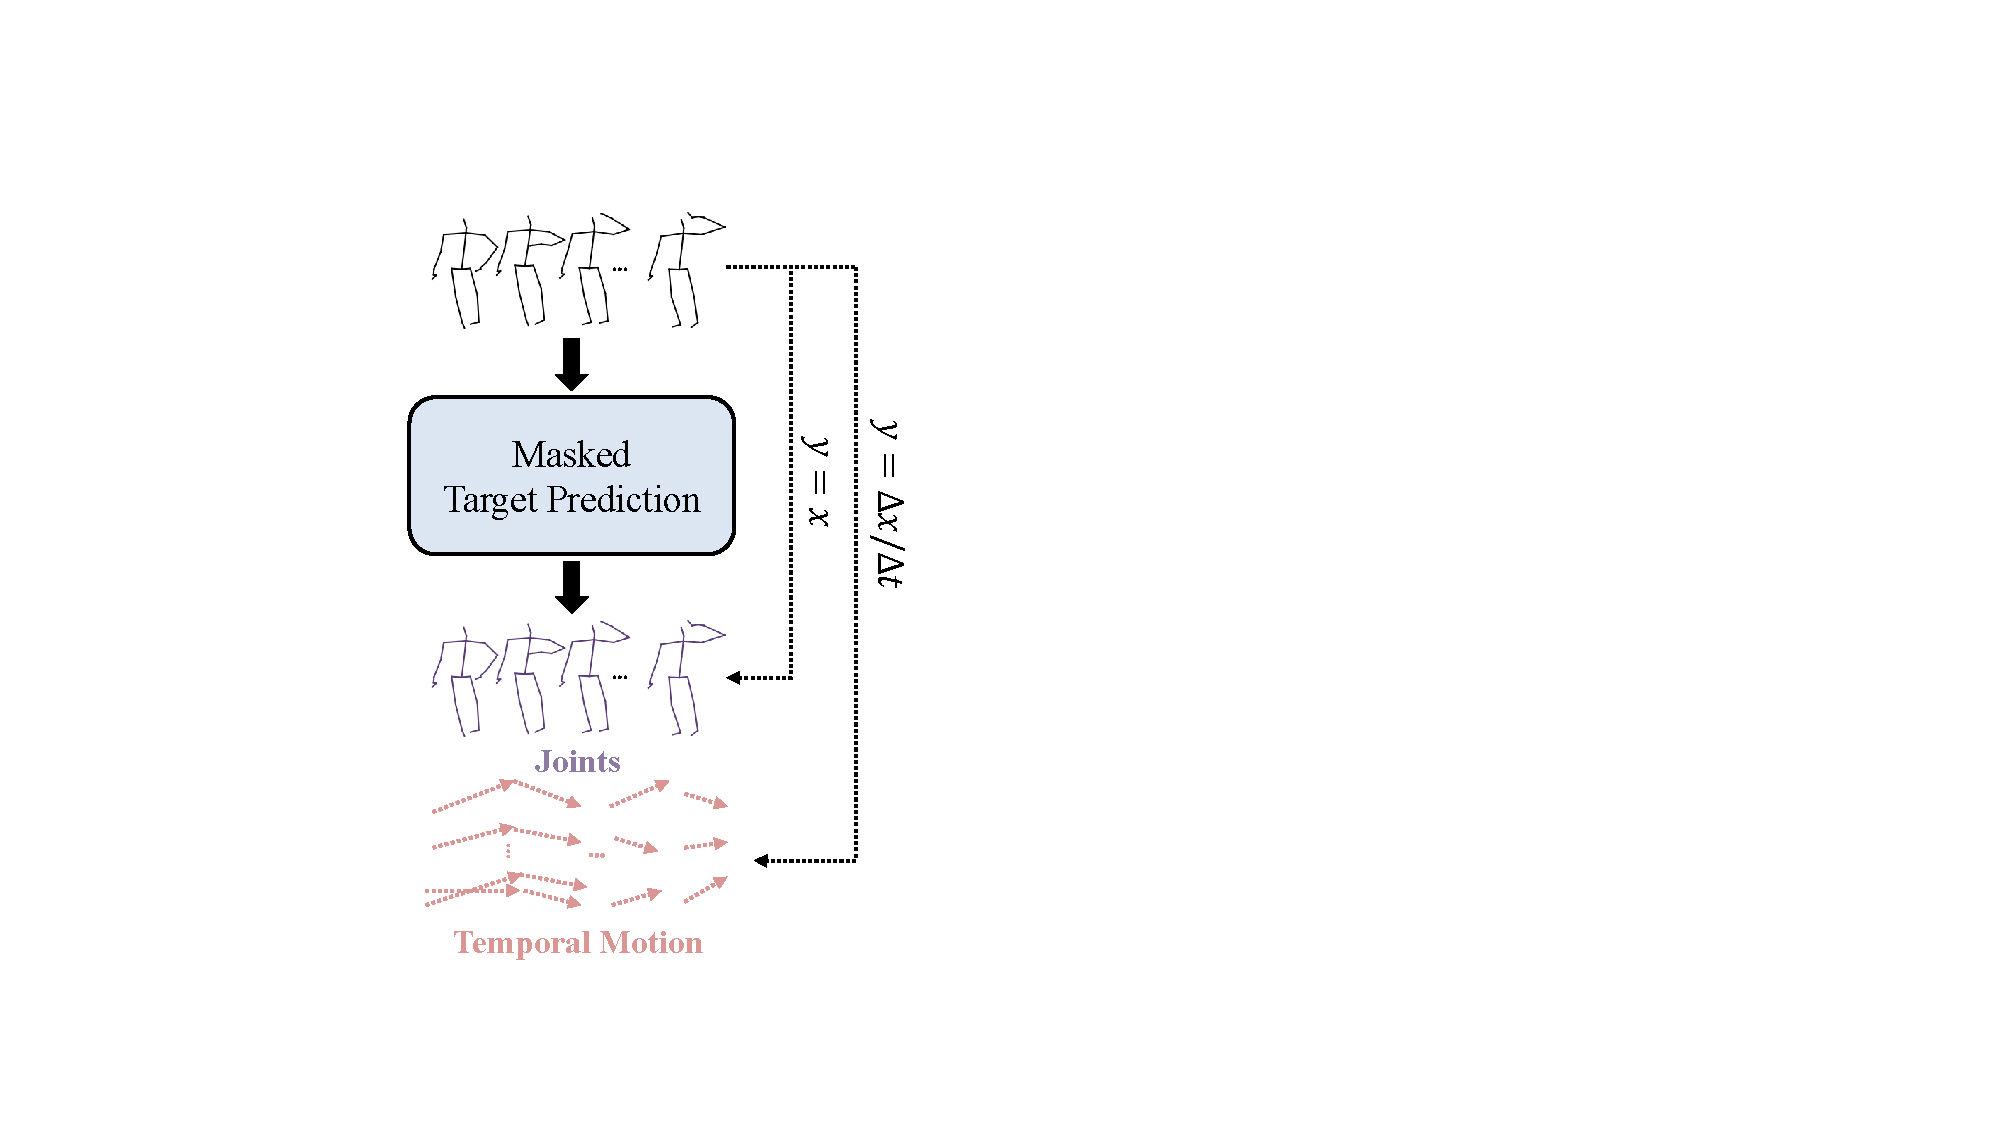
\includegraphics[width=1.0\linewidth]{figures/fig1_MAE.pdf}
		\caption{MAE-like}
		\label{fig1:MAE}
	\end{subfigure}
	\centering
	\begin{subfigure}{0.3\linewidth}
		\centering
		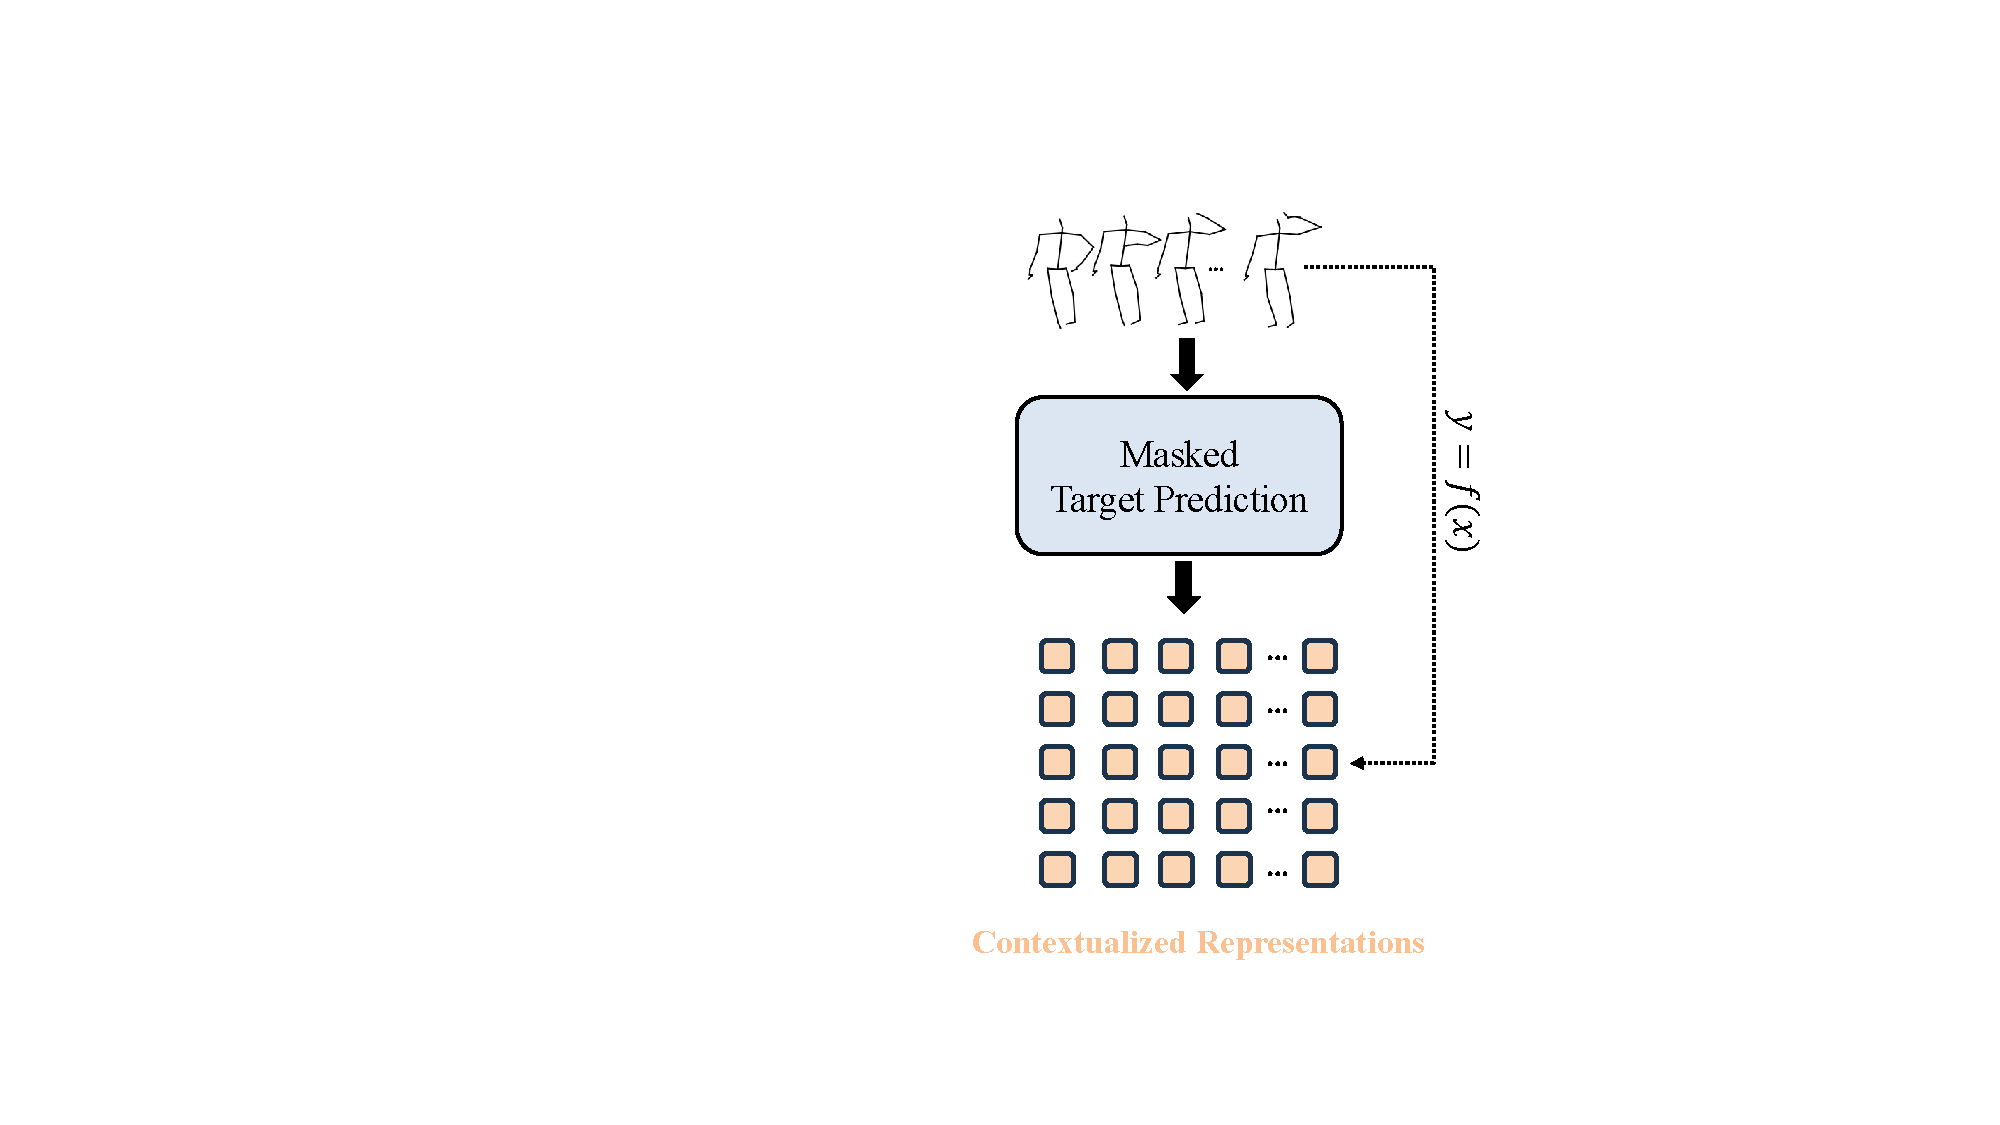
\includegraphics[width=1.0\linewidth]{figures/fig1_skeleton2vec.pdf}
		\caption{Skeleton2vec(Ours)}
		\label{fig1:skeleton2vec}
	\end{subfigure}
    \caption{
    A comparative illustration of the prediction targets between MAE-like methods (a) and
    ours Skeleton2vec (b). Skeleton2vec utilizes an teacher encoder $f(x)$ to generate
    globally contextualized representations as the prediction targets, instead of
    isolated joints or temporal motion with only local context.
    }
    \label{fig1}
\end{figure}

Human action recognition has significant applications in the real world, such as
security, human-robot interaction, and virtual reality. The development of depth
sensors and advancements in pose estimation algorithms \cite{2018OpenPose, fang2017rmpe, xu2020deep}
have propelled skeleton-based action recognition into a popular research topic,
owing to its computational efficiency, background robustness, and privacy preservation.
A series of fully-supervised skeleton-based human action recognition methods have
been developed using CNNs \cite{du2015skeleton,li2017skeleton}, RNNs \cite{liu2016spatio,zhang2017view},
and GCNs \cite{yan2018spatial,chen2021channel}. Despite their promising performance,
these methods rely on large amounts of manually annotated data, which is expensive,
labor-intensive, and time-consuming to obtain. This circumstance motivates us
to explore self-supervised representation learning for 3D actions.

Earlier works \cite{lin2020ms2l, nie2020unsupervised, su2020predict, zheng2018unsupervised}
have employed various pretext tasks, such as motion prediction, jigsaw puzzle recognition,
and masked reconstruction, to learn 3D action representations. Recently, contrastive
learning methods \cite{rao2021augmented, guo2022contrastive, moliner2022bootstrapped, lin2023actionlet}
have gained prominence. However, these methods often require carefully designed
data augmentations and tend to encourage the encoder to learn more global
representations, thereby neglecting local spatiotemporal information.
With the rise of transformer models \cite{vaswani2017attention}, self-supervised
pre-training methods based on masked prediction tasks have become mainstream in
visual representation learning \cite{rao2021augmented, guo2022contrastive, moliner2022bootstrapped, lin2023actionlet}.
Works like SkeletonMAE \cite{yan2023skeletonmae, wu2023skeletonmae} and MAMP \cite{mao2023masked} have
attempted to transfer MAE \cite{he2022masked} methods to the field of 3D action representation
learning, achieving promising results. However, these MAE-like methods inefficiently
utilize model capacity by focusing on low-level high-frequency details with
raw joint coordinates or temporal motion as learning targets, which is suboptimal
for modeling high-level spatiotemporal structures. We believe that using
higher-level prediction targets will guide the model to learn better representations
and improve pre-training performance.

Motivated by this idea, we propose Skeleton2vec, a simple and efficient self-supervised
framework for 3D action representation learning. Addressing the limitations of existing
MAE-like methods, as illustrated in \cref{fig1}, Skeleton2vec leverages contextualized
prediction targets. Following the work of data2vec \cite{baevski2022data2vec, baevski2023efficient},
we employ a teacher encoder that takes unmasked training samples to generate latent
contextualized representations as targets. We then use a student encoder, taking a
masked version of the sample as input, combined with an asymmetric decoder to
predict data representations at the masked positions. The entire model is based on the
vanilla transformer architecture. The self-attention mechanism ensures that the
constructed targets are contextualized, incorporating information from the entire
sample, making them richer than isolated targets (\eg raw joint coordinates)
or targets based on local context (\eg temporal motion).

Additionally, considering the strong spatiotemporal correlations in 3D skeleton sequences,
we propose a Motion-Aware Multi-Tube (MAMT) masking strategy. Initially, we divide the input skeleton
sequence along the temporal axis into multiple tubes, where frames within each tube share
a masking map to avoid information leakage from neighboring frames. This forces the model to
extract information from distant time steps for better prediction. We then guide the sampling
of masked joints based on the spatial motion intensity of body joints within each tube.
Joints with higher motion intensity will be masked with higher probability, allowing
the model to focus more on spatiotemporal regions with rich action semantics. Compared
to random masking, our method better utilizes the spatiotemporal characteristics and
motion priors of 3D skeleton sequences, effectively improving pre-training performance.

In summary, the main contributions of this work are three-fold:
\begin{itemize}
    \item{
        We propose the Skeleton2vec framework, which uses contextualized representations
        from a teacher encoder as prediction targets, enabling the learned representations
        to have stronger semantic associations.
    }
    \item{
        We introduce a motion-aware multi-tube masking strategy that performs persistent masking
        of joints within tubes based on spatial motion intensity, forcing the model to
        build better long-range spatiotemporal connections and focus on more semantic-rich regions.
    }
    \item{
        We validate the effectiveness of our method on three large-scale 3D skeleton-based
        action recognition datasets and achieve state-of-the-art results.
    }
\end{itemize}
\section{Related Work}
\label{sec:related}

% \subsection{Supervised Skeleton-based Action Recognition}
% How to effectively model skeleton action sequences using deep neural networks for
% supervised action recognition has been extensively explored
% \cite{ding2017investigation,du2015skeleton,li2017skeleton,liu2016spatio,zhang2017view,
% yan2018spatial,zhang2020semantics,chi2022infogcn,duan2022revisiting}.
% Earlier works typically use RNNs or CNNs to process skeletal data. 
% RNN-based methods \cite{liu2016spatio,zhang2017view} usually model skeletal data
% as a sequence of coordinate vectors, where each coordinate vector represents a
% human joint. CNN-based methods \cite{du2015skeleton,li2017skeleton} model skeletal
% data as a pseudo-image, where the time dimension (number of frames) and spatial
% dimension (number of joints) serve as the image width and height, and the joint
% coordinates as image channels. Despite achieving decent results, RNNs and CNNs do not
% well capture the inherent structure of skeletal data. Considering the natural
% spatiotemporal structure of skeletal data, ST-GCN \cite{yan2018spatial} models skeletal
% data as a graph structure and uses spatiotemporal graph convolutional networks to extract
% spatial and temporal features. ST-GCN \cite{yan2018spatial} has become the mainstream
% architecture for supervised action recognition due to its superior performance,
% and numerous improvements \cite{zhang2020semantics,chi2022infogcn,chen2021channel,
% shi2020skeleton} have been proposed, including dynamic graph topologies and various
% attention mechanisms. 
% With the rise of Transformer \cite{vaswani2017attention} models in CV
% \cite{dosovitskiy2020image,liu2021swin} and NLP \cite{devlin2018bert,lewis2019bart},
% some works \cite{qiu2022spatio,plizzari2021skeleton,shi2020decoupled} have attempted to
% introduce Transformers to skeleton-based action recognition.
% However, due to limited
% training data, vanilla Transformer \cite{vaswani2017attention} does not perform well.
% Thus, certain designs tailored for data characteristics are incorporated into
% Transformers to enhance inductive bias, such as temporal convolution \cite{qiu2022spatio},
% graph convolution \cite{plizzari2021skeleton,qiu2022spatio}, space-time separation
% \cite{shi2020decoupled}, etc, to alleviate the problem of limited training data and
% reduce overfitting.
% Earlier studies often use RNNs or CNNs for skeletal data processing. RNN-based
% methods \cite{liu2016spatio,zhang2017view} treat skeletal data as sequences of
% coordinate vectors representing human joints. CNN-based methods
% \cite{du2015skeleton,li2017skeleton} represent skeletal data as pseudo-images, with
% the time and spatial dimensions serving as image width and height, and joint
% coordinates as image channels. However, RNNs and CNNs fail to fully capture the
% inherent structure of skeletal data. To address this, ST-GCN \cite{yan2018spatial}
% models skeletal data as a graph structure, using spatiotemporal graph convolutional
% networks to extract spatial and temporal features. ST-GCN has emerged as the
% mainstream architecture for supervised action recognition and has seen various
% improvements \cite{zhang2020semantics,chi2022infogcn,chen2021channel,shi2020skeleton},
% including dynamic graph topologies and attention mechanisms.

% With the popularity of transformer models in computer vision
% \cite{dosovitskiy2020image,liu2021swin} and natural language processing
% \cite{devlin2018bert,lewis2019bart}, recent studies
% \cite{qiu2022spatio,plizzari2021skeleton,shi2020decoupled} have attempted to
% introduce transformers into skeleton-based action recognition.
% However, the performance of the vanilla transformer is limited by the lack of
% training data. Therefore, designs tailored for data characteristics are incorporated
% into transformers, such as temporal convolution \cite{qiu2022spatio},
% graph convolution \cite{plizzari2021skeleton,qiu2022spatio},
% and space-time separation \cite{shi2020decoupled},
% to enhance inductive bias and mitigate overfitting.

% Different from fully supervised training methods, this paper adopts the masked
% modeling paradigm to pretrain the original transformer model using a large amount of
% unsupervised data in order to learn a high-quality 3D motion representation for
% subsequent downstream tasks. Experimental results demonstrate that our pretraining
% enables the original transformer to unleash its inherent potential and achieve
% remarkable performance.

\subsection{Self-supervised Skeleton-based Action Recognition}
Previous studies \cite{zheng2018unsupervised,su2020predict,lin2020ms2l} on
self-supervised representation learning for skeleton-based action recognition
utilize various pretext tasks to capture motion context.
For instance, LongTGAN \cite{zheng2018unsupervised} leverages sequence reconstruction
to learn 3D action representations. P\&C \cite{su2020predict} employs a weak
decoder to enhance representation learning. MS2L \cite{lin2020ms2l} employs
motion prediction and jigsaw puzzle tasks. Yang et al. \cite{yang2021skeleton}
introduce a skeleton cloud colorization task.
Contrastive learning methods have gained prominence in 3D action representation learning
\cite{he2020momentum,grill2020bootstrap,rao2021augmented,guo2022contrastive,moliner2022bootstrapped,lin2023actionlet}.
AS-CAL \cite{rao2021augmented} and SkeletonCLR \cite{li20213d} utilize momentum encoder
and propose various data augmentation strategies. AimCLR \cite{guo2022contrastive} introduces
extreme augmentations. ActCLR \cite{lin2023actionlet} performs adaptive action modeling
on different body parts. Despite their remarkable results, contrastive learning methods
often overlook local spatio-temporal information, a crucial aspect for 3D action modeling.

The surge in popularity of transformers has led to the mainstream adoption of self-supervised
pretraining based on masked visual modeling for visual representation learning \cite{he2022masked,bao2021beit}.
SkeletonMAE \cite{wu2023skeletonmae} and MAMP \cite{mao2023masked} apply the Masked Autoencoder (MAE)
approach to 3D action representation learning. SkeletonMAE employs a skeleton-based encoder-decoder
transformer for spatial coordinate reconstruction, while MAMP introduces Masked Motion Prediction
to explicitly model temporal motion. In this study, we demonstrate that utilizing higher-level
contextualized representations as prediction targets for masked regions yields superior performance
compared to directly predicting raw joint coordinates or temporal motion.

\subsection{Masked Image Modeling}
BEiT \cite{bao2021beit} pioneered masked image modeling (MIM) for self-supervised pretraining
of visual models, aiming to recover discrete visual tokens from masked patches.
Subsequently, various prediction targets for MIM have been explored. MAE \cite{he2022masked}
and SimMIM \cite{xie2022simmim} treat MIM as a denoising self-reconstruction task, utilizing
raw pixels as the prediction target. MaskFeat \cite{wei2022masked} replaces pixels with HOG
descriptors to enable more efficient training and achieve superior results. PeCo \cite{dong2023peco}
introduces a perceptual loss during dVAE training to generate semantically richer discrete
visual tokens, surpassing BEiT.
These works demonstrate superior performance by utilizing
higher-level and semantically richer prediction targets in MIM.
To further enhance performance,
data2vec \cite{baevski2022data2vec,baevski2023efficient} employs self-distillation to
leverage latent target representations from the teacher model output at masked positions.
Compared to isolated targets like visual tokens or pixels, these contextualized representations
encompass relevant features from the entire image, enabling improved performance.

In this research, we introduce the data2vec framework into self-supervised pretraining of
skeleton sequences, utilizing latent contextualized target representations from the teacher
model to guide the student model in learning more effective 3D action representations.


\section{Method}
\subsection{Overview}

\begin{figure}[tb]
	\centering
	\begin{subfigure}{0.49\linewidth}
		\centering
		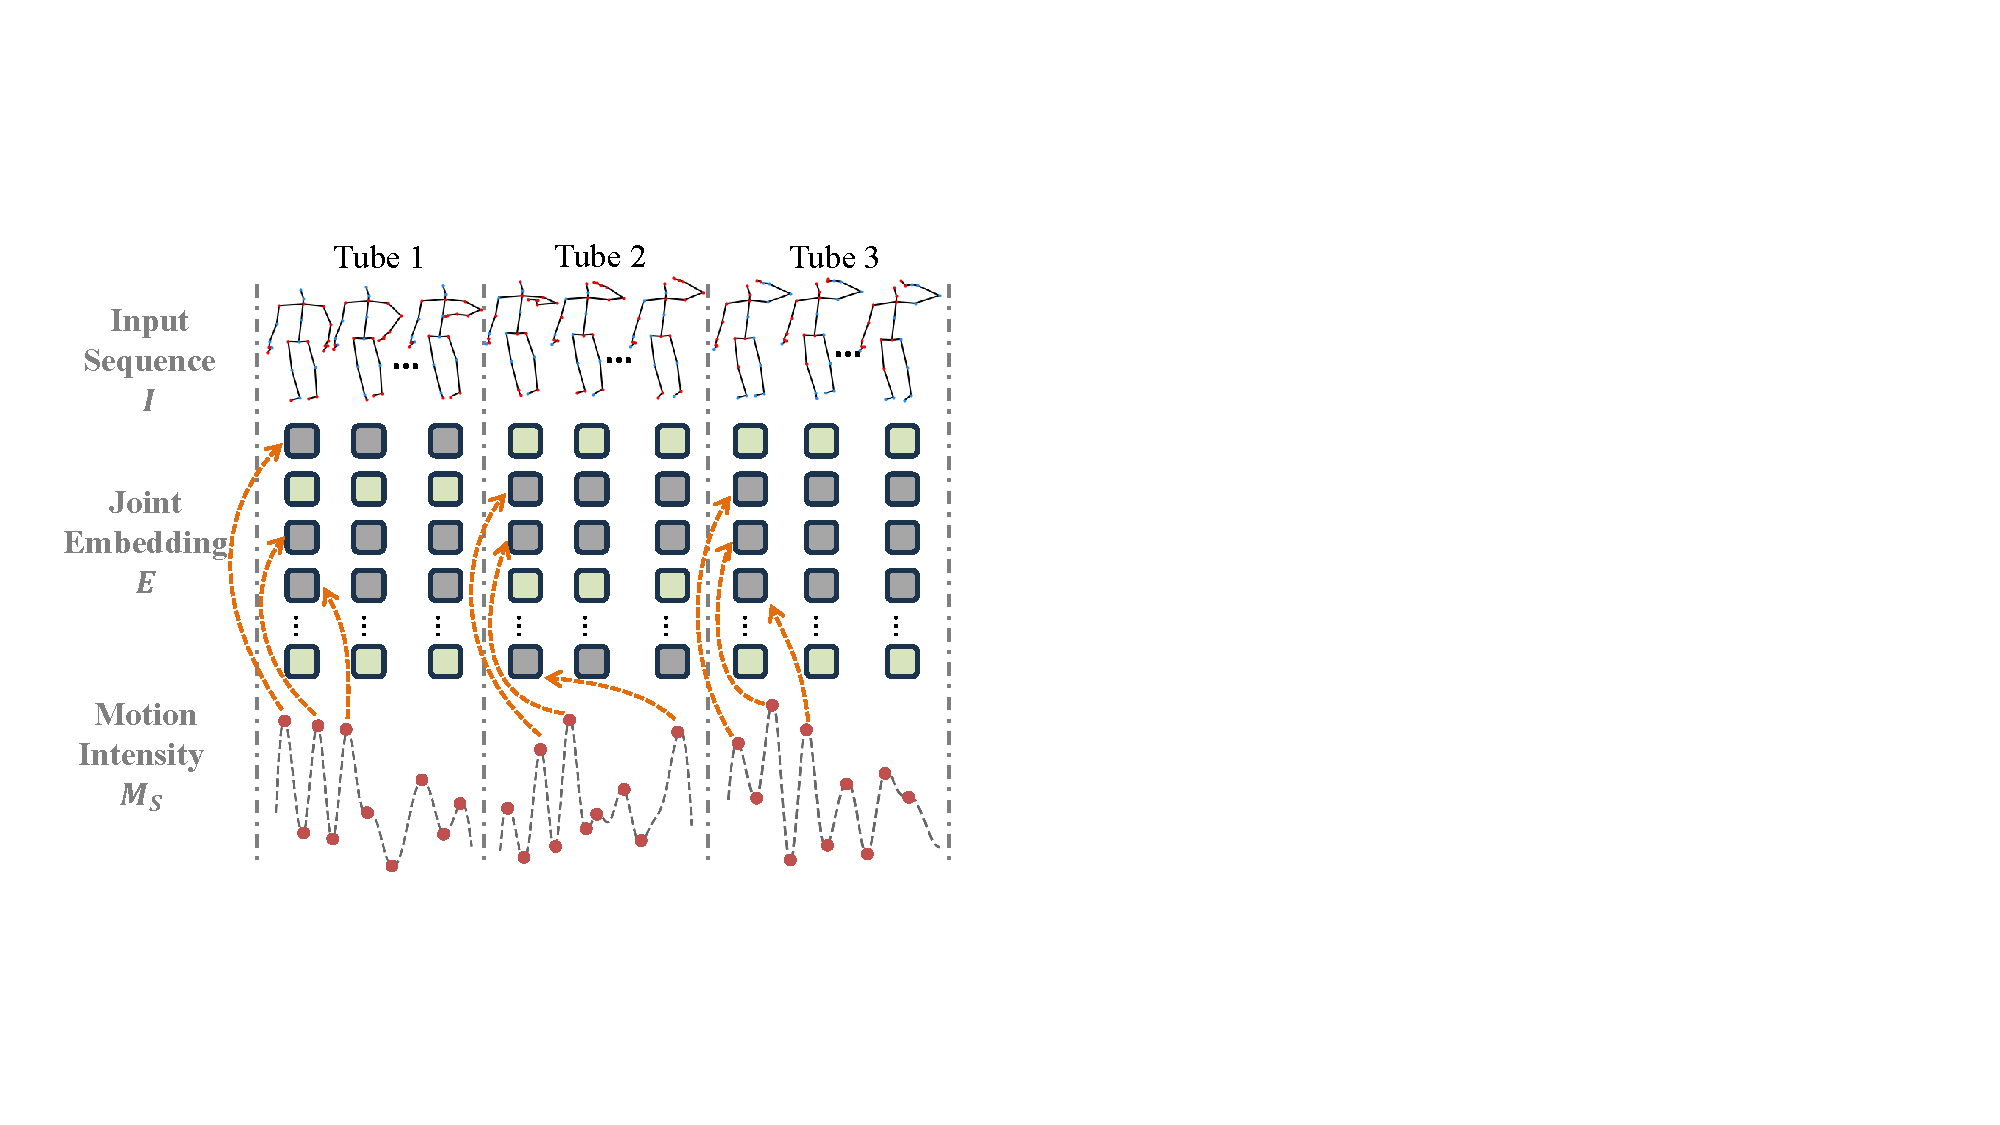
\includegraphics[width=0.95\linewidth]{figures/fig2_motion_aware_tube_masking.pdf}
		\caption{Motion-Aware Multi-Tube Masking}
		\label{fig2:motion_aware_tube_masking}
	\end{subfigure}
	\centering
	\begin{subfigure}{0.49\linewidth}
		\centering
		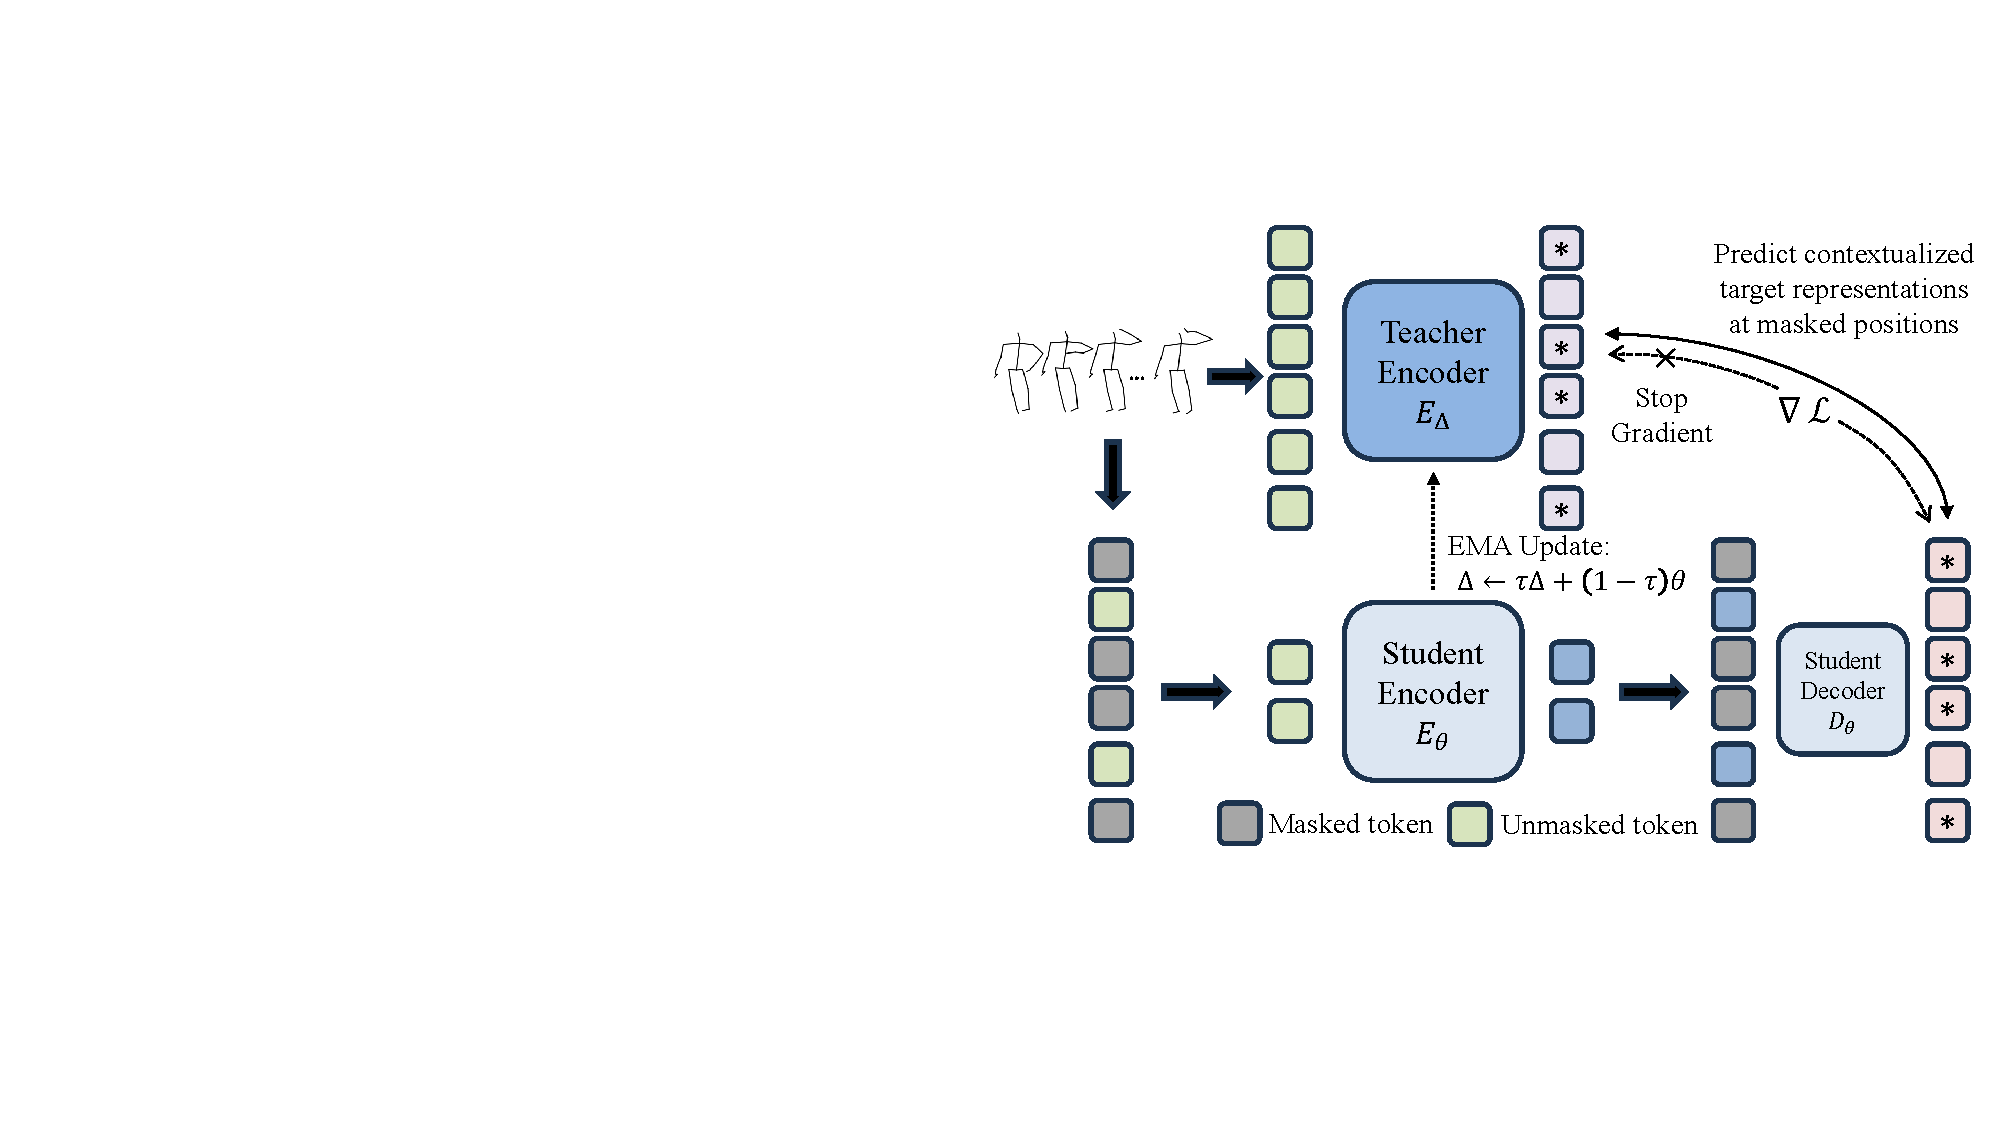
\includegraphics[width=0.95\linewidth]{figures/fig2_skeleton2vec.pdf}
		\caption{Skeleton2vec}
		\label{fig2:skeleton2vec}
	\end{subfigure}
    \caption{
    The overall pipeline of the proposed Skeleton2vec framework.
    We adopt the motion-aware multi-tube masking strategy (a) to guide the masking process,
    which prevents information leakage between adjacent frames and allows the model
    to focus more on semantically rich regions of motion. Subsequently, the teacher
    encoder $E_{\Delta}$ receives unmasked samples to construct latent contextualized targets,
    while the student encoder $E_{\theta}$ receives masked versions of the samples
    and predicts corresponding representations at the masked positions.
    }
    \label{fig2}
    \vspace{-8pt}
\end{figure}

The overall framework of Skeleton2vec is shown in \cref{fig2}.
It takes a skeleton sequence $I \in \mathbb{R}^{T_{s} \times V \times C_{s}}$ as
input, where $T_{s}$ is the the number of frames,
$V$ is the number of joints, and $C_{s}$ is the
the coordinates of joints.
Similar to most visual transformers \cite{dosovitskiy2020image},
the skeleton sequence is first divided into fixed-size patches and then linearly
transformed into patch embedding $E \in \mathbb{R}^{T_{e} \times V \times C_{e}}$.
After that, we employ the motion-aware multi-tube masking strategy to guide the masking of
joints. The teacher model constructs the full contextualized prediction targets
using unmasked training samples, while the student model receives the masked version
of the samples and predicts corresponding representations at the masked positions.

As our student model, we adopt an asymmetric encoder-decoder architecture, where the
encoder operates solely on non-masked tokens. The lightweight decoder inserts masked
tokens into the latent representations outputted by the encoder, forming a full set
for predicting the targets.
The teacher encoder shares the same model structure as the student. After accomplishing
the aforementioned pre-training task, the teacher encoder is retained for downstream task fine-tuning.

\subsection{Model Architecture}
\noindent \textbf{Encoder:}
Following MAMP \cite{mao2023masked}, we first divide the raw skeleton sequence
$I \in \mathbb{R}^{T_{s} \times V \times C_{s}}$ into non-overlapping segments
$I' \in \mathbb{R}^{T_{e} \times V \times (l \cdot C_{s})}$, where $T_{e}=T_{s}/l$
and $l$ is the length of each segment.
A trainable linear projection is then applied to each joint to obtain the embedding:
\begin{equation}
    \label{eq:joint_embedding_1}
    E_{j} = \text{LinearProj}(I') \in \mathbb{R}^{T_{e} \times V \times C_{e}},
\end{equation}
where $C_{e}$ represents the dimension of the embedding.
Temporal positional embedding $E_{t} \in \mathbb{R}^{T_{e} \times 1 \times C_{e}}$
and spatial positional embedding $E_{s} \in \mathbb{R}^{1 \times V \times C_{e}}$
are then added to the joint embedding to yield the final input:
\begin{equation}
    \label{eq:joint_embedding_2}
    E = E_{j} + E_{t} + E_{s},
\end{equation}

For the teacher encoder, the entire set is flattened as input $E^{T} \in \mathbb{R}^{N_{T} \times C_{e}}$,
where $N_{T}=T_{e} \times V$ represents the total number of tokens in the
skeleton sequence. For the student encoder, most tokens are masked, and
only the unmasked tokens are utilized as input, flattened as $E^{S} \in \mathbb{R}^{N_{S} \times C_{e}}$,
where $N_{S}=T_{e} \times V \times (1-m)$ denotes the number of visible tokens,
and $m$ is the masking ratio. 
Subsequently, $L_{e}$ layers of vanilla transformer blocks are applied to extract
latent representations. Each block comprises a multi-head self-attention (MSA)
module and a feed-forward network (FFN) module. Residual connections are employed
within each module, followed by layer normalization (LN).

\noindent \textbf{Decoder:} The decoder input
$D \in \mathbb{R}^{T_{e} \times V \times C_{e}}$ contains the full set of tokens,
including the latent representations of visible encoded tokens $Z^{S}_{e}$ and the inserted masked tokens.
Each masked token is represented by a shared learnable vector $E_{M} \in \mathbb{R}^{C_{e}}$,
indicating missing information to be predicted at that position. Similar to the
encoder, spatial positional embedding $E'_{s}$ and temporal positional embedding
$E'_{t}$ are added to all tokens to assist masked tokens in locating their positions.
The decoder employs an additional $L_{d}$ layers of transformer blocks for masked prediction.

\subsection{Contextualized Target Prediction}
Rather than relying on isolated raw joints or temporal motion with limited local context, we employ a
transformer-based teacher encoder to construct globally contextualized prediction targets,
thereby introducing a diverse training task.

\noindent \textbf{Contextualized Target Representations:}
We extract features from the output of each FFN block in every layer of the
teacher encoder and average them to form our training targets. Following data2vec 2.0
\cite{baevski2023efficient}, the features from each layer are normalized with
instance normalization \cite{ulyanov2016instance} before averaging.
Finally, the averaged features are normalized by layer normalization to serve as
the prediction targets. Normalizing the targets helps prevent the model from
collapsing to a trivial solution, and also prevents any single layer's features
from dominating. The generation of the target representations can be formulated as:
\begin{equation}
    \label{eq:target_rep}
    \begin{aligned}
        Y' &= \frac{1}{L_e}\sum_{l=1}^{L_e} \text{IN}(Z_l^T), \\
        Y &= \text{LN}(Y'),
    \end{aligned}
\end{equation}
where IN and LN refer to instance normalization and layer normalization, respectively.
$Z_l^T$ denotes the output of the FFN block in the $l^{th}$ layer of the teacher encoder.

\noindent \textbf{Target Prediction:}
Given the output $H_d$ of the student decoder, we employ an additional linear prediction head to
regress the contextualized target representations of the teacher:  
\begin{equation}
    \label{eq:target_pred}
    \hat{Y} = \text{LinearPred}(H_d),
\end{equation}

Finally, we adopt L2 loss as our learning objective, calculating loss only for the
masked positions:
\begin{equation}
    \label{eq:loss}
    \mathcal{L} = \frac{1}{|\mathcal{M}|}\sum_{i \in \mathcal{M}}||Y_i - \hat{Y}_i||_2^2,
\end{equation}
where $\mathcal{M}$ denotes the set of masked positions.

\noindent \textbf{Teacher Parameterization:}
The student model weights $\theta$ are updated through backpropagation on the loss
gradients. The teacher model weights $\Delta$ are initialized to be the same as the
student weights and parameterized during training by taking an exponentially moving
average (EMA) of the student weights:  
\begin{equation}
    \label{eq:ema}
    \Delta \leftarrow \tau\Delta + (1-\tau)\theta,
\end{equation}
where $\tau$ is a hyperparameter controlling the update frequency of the teacher
weights using a linearly increasing schedule, gradually increasing from an initial
value $\tau_0$ to 1 throughout training.

\subsection{Motion-Aware Multi-Tube Masking}
\label{sec:motion-aware_tube_masking}
We propose the motion-aware multi-tube masking strategy to address the issue of high
spatiotemporal correlations in skeleton sequences.

\begin{wrapfigure}{r}{0.5\textwidth}
    \vspace{-10pt}
  \centering
  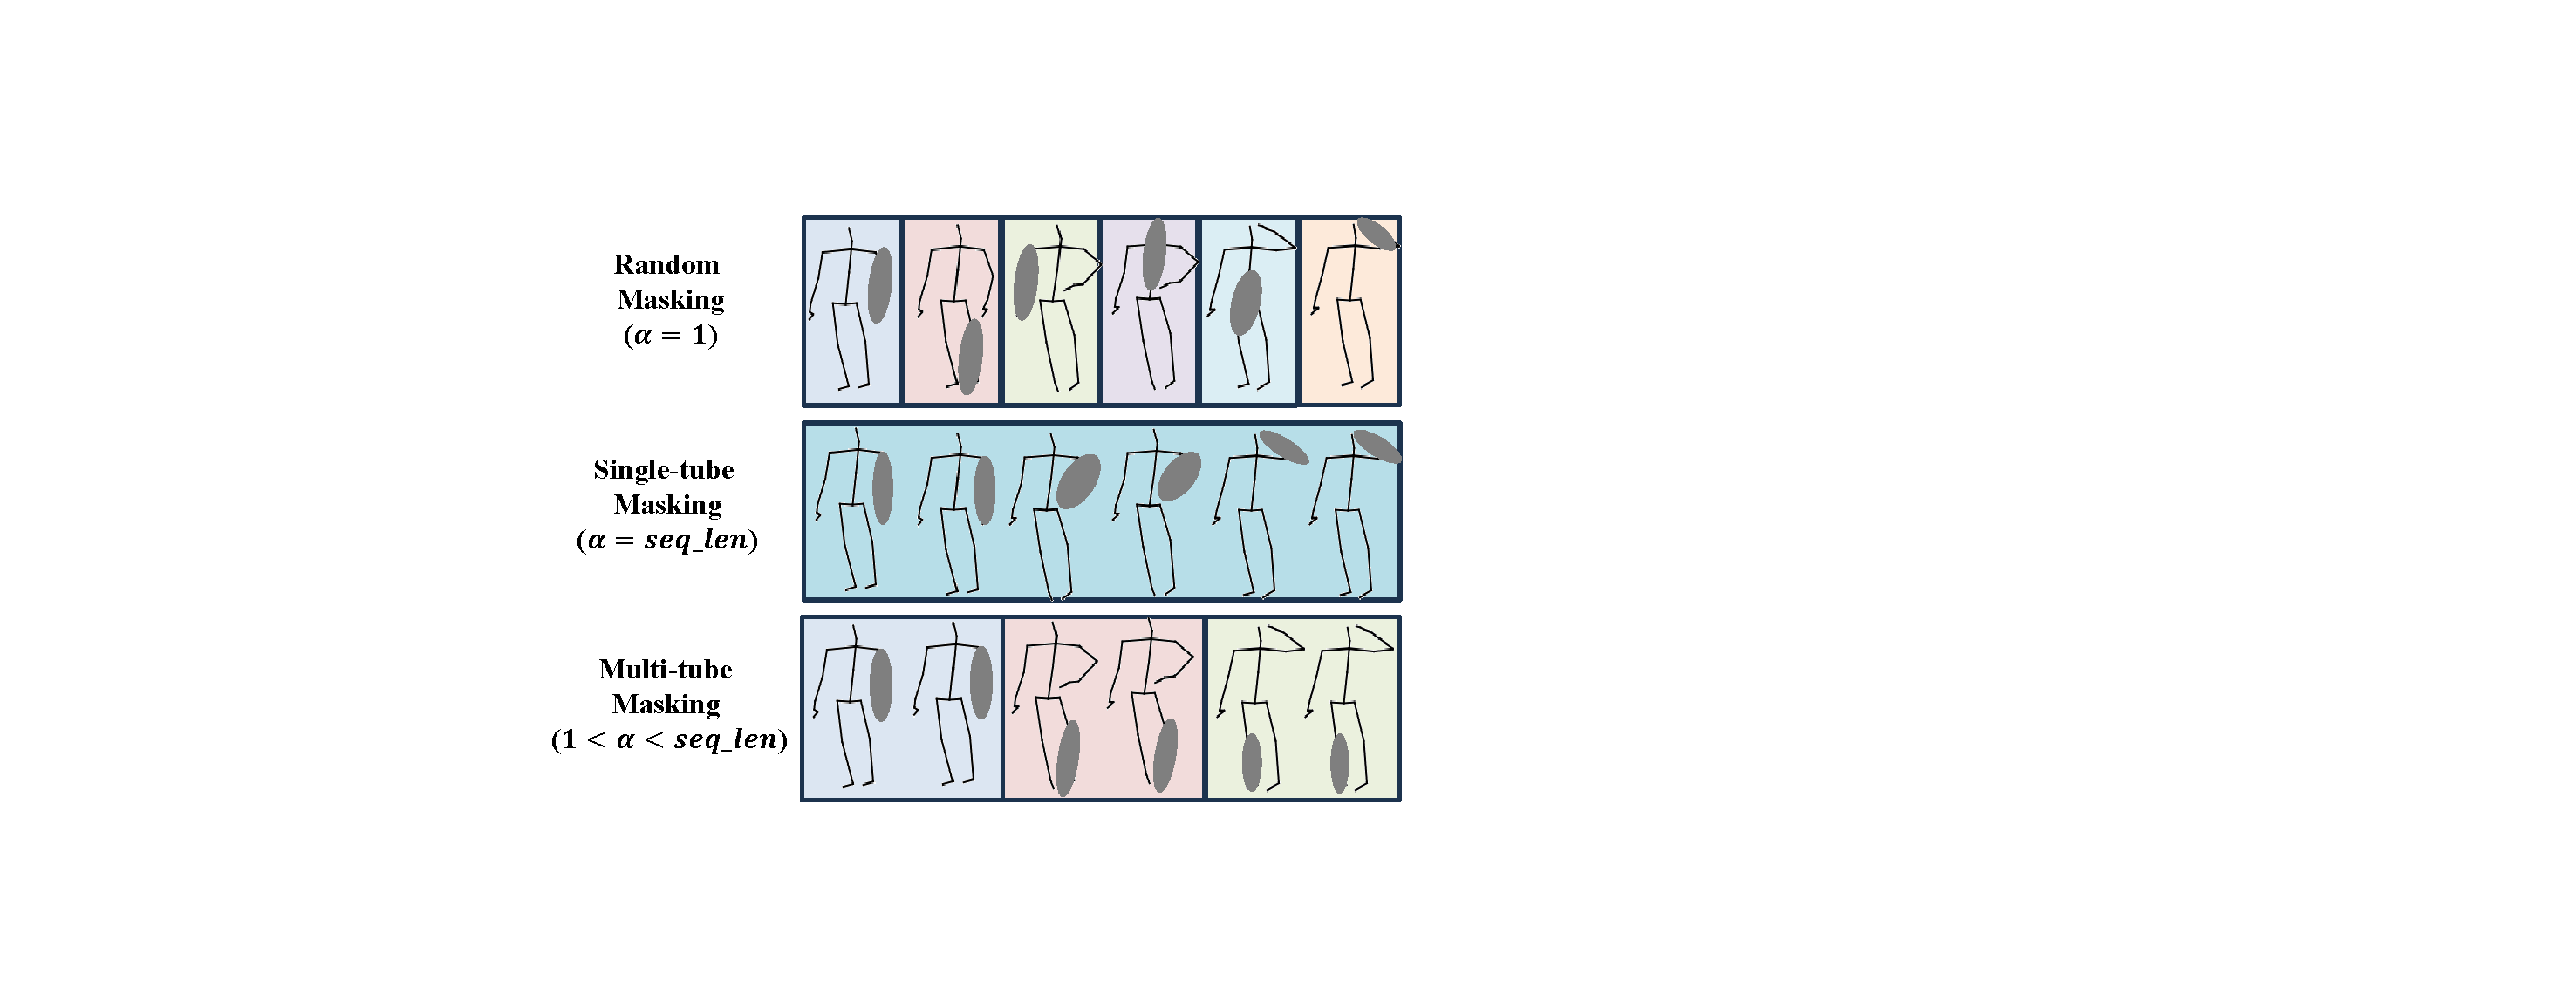
\includegraphics[width=0.5\textwidth]{figures/fig_masking_cmp.pdf} % 更换图片路径
  \caption{
    Intuitive comparison of different masking strategies.
    The gray shade represents the masked region, with different
    colors denoting different masking maps, while $seq\_len$
    indicates the length of the sequence.
  }
    \label{fig:masking_cmp}
    \vspace{-10pt}
\end{wrapfigure}

\noindent \textbf{Multi-Tube Division:}
The tube masking strategy, initially introduced by VideoMAE \cite{tong2022videomae},
considers the entire video sequence along the temporal axis as a single tube,
sharing the same masking map across different frames. This mitigates the information
leakage issue between adjacent frames.
Although the skeleton sequence is derived from the
video, directly applying this single-tube
masking strategy to skeleton data is suboptimal due to the inherent structural differences.
In video data, the basic units for masking are image patches in each frame. Due to scene
motion or camera viewpoint changes, a masked body part like the hand in the first frame
may find its correspondence in unmasked regions in later frames far apart, which facilitates
long-range dependency modeling.
In contrast, the basic units for masking in skeleton sequences
are the joints in each skeleton frame, where the same-order joints have explicit correspondence
across frames. As a result, a body part masked in the first skeleton frame will remain
masked in all frames, causing a complete loss of information
for that part (as shown in the second row of \cref{fig:masking_cmp}), which makes
the masked prediction task overly difficult and harms the model's learning capability.
To address this, as illustrated in \cref{fig2:motion_aware_tube_masking} and \cref{fig:masking_cmp},
we empirically divide the skeleton sequence along the time axis into multiple tubes
instead of one tube. Each tube shares the same masking map to force the model to extract
information from farther time steps, while different tubes use different masking maps
to avoid joints being masked throughout.
The tube division can be represented as:
\begin{equation}
    \label{eq:deviding_tubes}
    E'=\text{Reshape}(E) \in \mathbb{R}^{N \times \alpha \times V \times C_{e}}, 
\end{equation}

\noindent where $\alpha$ is tube length and $N=\frac{T_{e}}{\alpha}$ is number of tubes.
It can be observed in \cref{fig:masking_cmp} that random
masking samples a different masking map for each frame,
single-tube masking shares a single masking map
across all frames, while our multi-tube masking is a compromise between the two,
sharing the masking map only among several adjacent frames.
This approach mitigates information leakage while encouraging the model to
establish long-range spatiotemporal relationships.
% The comparison between random masking, single-tube masking, and our
% multi-tube masking is visually depicted in \cref{fig:masking_cmp}.

\noindent \textbf{Motion-Aware Sampling:}
Regions with larger motion intensity intuitively contain richer semantic information
about actions. Therefore, we utilize the spatial motion intensity of each human body
joint within a tube as empirical guidance to generate the masking map.

Specifically, we first extract the corresponding motion sequence
$M \in \mathbb{R}^{T_{s} \times V \times C_{s}}$ from the input skeleton sequence
$I \in \mathbb{R}^{T_{s} \times V \times C_{s}}$ by calculating temporal differences
of corresponding joint coordinates between adjacent frames:
\begin{equation}
    \label{eq:motion}
    M_{i,:,:} = \begin{cases} 
    I_{i+1,:,:}-I_{i,:,:}, & i \in 0, \dots, T_{s}-1\\
    0, & i=T_{s}  
\end{cases}
\end{equation}

Similar to joint embedding in the encoder, we reshape $M$ into non-overlapping
segments $M' \in \mathbb{R}^{T_{e} \times V \times (l \cdot C_{s})}$ to match the
shape of input sequence $I'$. We then calculate the motion intensity of each joint
within a segment as:
\begin{equation}  
    \label{eq:motion_intensity}
    S_{i,:} = \sum_{k=0}^{l\cdot C_{s}}|M'_{i,:,k}| \in \mathbb{R}^{T_{e} \times V}, \quad i=0,\dots,T_{e}
\end{equation}

Afterwards, we compute the spatial motion intensity of each body joint within a tube,
normalizing it along the spatial dimension:  
\begin{equation}
    \label{eq:tube_motion_intensity_norm}
    \begin{aligned}
        T_{i,:} &= \sum_{j=i}^{i+\alpha}S_{j,:} \in \mathbb{R}^{N \times V}, \quad &i=0,\dots,N \\
        T'_{i,:} &= T_{i,:} / \text{max}(T_{i,:}), \quad &i=0,\dots,N  
    \end{aligned}
\end{equation}

Finally, we utilize the normalized spatial motion intensity to generate a unique
masking map for each tube:
\begin{equation} 
    \label{eq:mask_sampling}
    \begin{aligned}
        p &= \eta + \beta \cdot T', \quad &\eta \sim U(0,1) \\  
        \mathcal{M}_{i} &= \text{argsort}(p_{i,:})[-K:], \quad &i=0,\dots,N
    \end{aligned}
\end{equation}

\noindent where $\eta$ is random noise drawn from a uniform distribution between
0 and 1, $\beta$ is a hyperparameter controlling the influence of spatial motion
intensity on sampling, $\mathcal{M}_{i}$ is the masking map for $i^{th}$ tube,
$K=V\times (1-m)$ is the number of joints to be masked, and $m$ is the masking ratio.
By customizing motion-aware masking maps for each tube, the model is encouraged
to focus more on semantically richer regions, leading to improved spatiotemporal representations.



\section{Experiments}
\subsection{Datasets}
We evaluate our method on three large-scale 3D skeleton-based action recognition
datasets: NTU RGB+D 60, NTU RGB+D 120, and PKU Multi-Modality Dataset (PKUMMD).

NTU RGB+D 60 \cite{shahroudy2016ntu} contains 56,880 skeleton sequences across 60
action categories performed by 40 subjects. We follow the recommended cross-subject
and cross-view evaluation protocols. For cross-subject, sequences from 20 subjects
are used for training and the rest are used for testing. For cross-view, training
samples are from cameras 2 and 3, while testing samples are from camera 1. 

NTU RGB+D 120 \cite{liu2019ntu} is an extension of NTU RGB+D 60 with 114,480
skeleton sequences across 120 action categories performed by 106 subjects.
The authors also propose a more challenging cross-setup evaluation protocol, where
sequences are divided into 32 setups based on camera distance and background. Samples
from 16 setups are used for training and the rest are used for testing.

PKUMMD \cite{liu2017pku} contains nearly 20,000 skeleton sequences across 52 action
categories. We adopt the cross-subject protocol, where training and testing sets are
split based on subject ID. PKUMMD consists of two parts: PKU-I and PKU-II. PKU-II is
more challenging due to larger view variations that introduce more skeleton noise.
For PKU-II, there are 5,332 sequences for training and 1,613 for testing.

\subsection{Settings}
\noindent \textbf{Data Processing:}
We employed the data preprocessing method from DG-STGCN \cite{duan2022dg} to apply
uniform sampling to a given skeleton sequence, generating subsequences as training
samples. The number of frames $T_{s}$ for sampling is set to 90.
During the training, we applied random rotation as data augmentation on the
sampled subsequences to enhance robustness against view variation. During the testing,
we averaged the scores of 10 subsequences to predict the class.

\noindent \textbf{Network Architecture:}
We adopted the same network architecture setting as MAMP \cite{mao2023masked}, with the
encoder layers $L_{e}$ set to 8, decoder layers $L_{d}$ set to 3, embedding dimension
set to 256, the number of heads in the multi-head self-attention module set to 8, and
the hidden dimension of the feed-forward network set to 1024. For Joint Embedding,
the length $l$ of each segment is set to 3.

\noindent \textbf{Pre-training:}
In the pre-training, the initial value of the EMA parameter $\tau$ is set to 0.9999.
The masking ratio $m$ of the input sequence is set to 90\%.
The tube length $\alpha$ for motion-aware multi-tube masking is set to 5,
and the sampling parameter $\beta$ is set to 0.1. We utilized the AdamW optimizer
with weight decay of 0.05 and betas (0.9, 0.95). The model was trained for a total of
600 epochs, with the learning rate linearly increasing to 1e-3 during the first 20
warmup epochs, and then decaying to 1e-5 according to a cosine decay schedule.
Our model was trained on 2 RTX 4090 GPUs, with a total batch size of 128.

\begin{table}[tb] \scriptsize
    \caption{
      Performance comparison in linear evaluation protocol
      on NTU 60, NTU 120, and PKU MMD datasets.
      \textit{Single-stream} refers to Joint,
      while \textit{Three-stream} denotes Joint+Motion+Bone.
    }
    \centering
    \setlength{\tabcolsep}{4pt} % 增大列与列之间的水平间距
    \begin{tabular}{l c c c c c c}
      \toprule
      \multirow{2}{*}{Method} &
      \multirow{2}{*}{Input} &
      \multicolumn{2}{c}{NTU 60} &
      \multicolumn{2}{c}{NTU 120} &
      PKU II\\
      % & & XSub(\%) & XView(\%) & XSub(\%) & XSet(\%) & XSub(\%) \\
      & & XSub & XView & XSub & XSet & XSub \\
      \midrule
      \rowcolor{Gray!20} \multicolumn{7}{l}{\textit{Other pretext tasks:}} \\
      LongTGAN \cite{zheng2018unsupervised} & Single-stream & 39.1 & 48.1 & - & - & 26.0 \\
      P\&C \cite{su2020predict} & Single-stream & 50.7 & 75.3 & 42.7 & 41.7 & 25.5 \\
      \midrule
      \rowcolor{Gray!20} \multicolumn{7}{l}{\textit{Contrastive Learning:}} \\
      CrosSCLR \cite{li20213d} & Three-stream & 77.8 & 83.4 & 67.9 & 66.7 & 21.2 \\
      AimCLR \cite{guo2022contrastive} & Three-stream & 78.9 & 83.8 & 68.2  & 68.8 & 39.5 \\
      CPM \cite{zhang2022contrastive} & Single-stream & 78.7 & 84.9 & 68.7 & 69.6 & - \\
      PSTL \cite{Zhou2023SelfsupervisedAR} & Three-stream & 79.1 & 83.8 & 69.2 & 70.3 & 52.3 \\
      CMD \cite{mao2022cmd} & Single-stream & 79.4 & 86.9 & 70.3 & 71.5 & - \\
      HaLP \cite{shah2023halp} & Single-stream & 79.7 & 86.8 & 71.1 & 72.2 & 43.5 \\
      HiCo-Transformer \cite{hico2023} & Single-stream & 81.1 & 88.6 & 72.8 & 74.1 & 49.4 \\
      SkeAttnCLR \cite{Hua2023SkeAttnCLR} & Three-stream & 82.0 & 86.5 & 77.1 & 80.0 & 55.5 \\
      ActCLR \cite{lin2023actionlet} & Three-stream & 84.3 & 88.8 & 74.3 & 75.7 & - \\
      \midrule
      \rowcolor{Gray!20} \multicolumn{7}{l}{\textit{Masked Prediction:}} \\
      SkeletonMAE \cite{yan2023skeletonmae} & Single-stream & 74.8 & 77.7 & 72.5 & 73.5 & 36.1 \\
      MAMP \cite{mao2023masked} & Single-stream & 84.9 & 89.1 & 78.6 & 79.1 & 53.8 \\
      \textbf{Skeleton2vec(Ours)} & Single-stream & \textbf{85.7} & \textbf{90.3} & \textbf{79.7} & \textbf{81.3} & \textbf{55.6} \\
      \bottomrule
    \end{tabular}
    \label{tab:linear}
    \vspace{-15pt}
\end{table}

\begin{table}[tb] \scriptsize
    \caption{
      Performance comparison in the semi-supervised protocol on NTU 60 datasets.
      We averaged the results of five runs as the final performance.
    }
    \centering
    \setlength{\tabcolsep}{4pt} % 增大列与列之间的水平间距
    \begin{tabular}{l c c c c c}
      \toprule
      \multirow{3}{*}{Method} &
      \multirow{2}{*}{Input} &
      \multicolumn{4}{c}{NTU 60} \\
      & & \multicolumn{2}{c}{XSub} & \multicolumn{2}{c}{XView} \\
      & & (1\%) & (10\%) & (1\%) & (10\%) \\
      \midrule
      \rowcolor{Gray!20} \multicolumn{6}{l}{\textit{Other pretext tasks:}} \\
      LongTGAN \cite{zheng2018unsupervised} & Single-stream & 35.2 & 62.0 & - & - \\
      MS2L \cite{lin2020ms2l} & Single-stream & 33.1 & 65.1 & - & - \\
      \rowcolor{Gray!20} \multicolumn{6}{l}{\textit{Contrastive Learning:}} \\
      % ISC \cite{thoker2021skeleton} & Single-stream & 35.7 & 65.9 & 38.1 & 72.5 \\
      3s-CrosSCLR \cite{li20213d} & Three-stream & 51.1 & 74.4 & 50.0 & 77.8 \\
      % 3s-Colorization \cite{yang2021skeleton} & Three-stream & 48.3 & 71.7 & 52.5 & 78.9 \\
      3s-Hi-TRS \cite{chen2022hierarchically} & Three-stream & 49.3 & 77.7 & 51.5 & 81.1 \\
      3s-AimCLR \cite{guo2022contrastive} & Three-stream & 54.8 & 78.2 & 54.3 & 81.6 \\
      3s-CMD \cite{mao2022cmd} & Three-stream & 55.6 & 79.0 & 55.5 & 82.4 \\
      CPM \cite{zhang2022contrastive} & Three-stream & 56.7 & 73.0 & 57.5 & 77.1 \\
      3s-HYSP \cite{franco2023hyperbolic} & Three-stream & - & 80.5 & - & 85.4 \\
      3s-SkeAttnCLR \cite{Hua2023SkeAttnCLR} & Three-stream & 59.6 & 81.5 & 59.2 & 83.8 \\
      \rowcolor{Gray!20} \multicolumn{6}{l}{\textit{Masked Prediction:}} \\
      SkeletonMAE \cite{wu2023skeletonmae}& Single-stream  & 54.4 & 80.6 & 54.6 & 83.5 \\
      MAMP \cite{mao2023masked} & Single-stream & 66.0 & 88.0 & 68.7 & 91.5 \\
      \midrule
      \textbf{Skeleton2vec(Ours)} & Single-stream & \textbf{75.7} & \textbf{89.2} & \textbf{76.2} & \textbf{92.9} \\
      \bottomrule
    \end{tabular}
    \label{tab:semi-supervised}
    \vspace{-14pt}
\end{table}

\begin{table}[tb] \scriptsize
    \caption{
      Performance comparison in fine-tuning protocol on NTU 60 and NTU 120 datasets.
      The best results are shown in bold, and the second-best results
      are highlighted with an underline.
    }
    \centering
    \setlength{\tabcolsep}{4pt} % 增大列与列之间的水平间距
    \begin{tabular}{l c c c c c c}
      \toprule
      \multirow{2}{*}{Method} &
      \multirow{2}{*}{Input} &
      \multirow{2}{*}{Backbone} &
      \multicolumn{2}{c}{NTU 60} &
      \multicolumn{2}{c}{NTU 120} \\
      & & & XSub & XView & XSub & XSet \\
      \midrule
      \rowcolor{Gray!20} \multicolumn{7}{l}{\textit{Other pretext tasks:}} \\
      Colorization \cite{yang2021skeleton} & Three-stream & DGCNN & 88.0 & 94.9 & - & - \\
      Hi-TRS \cite{chen2022hierarchically} & Three-stream & Transformer & 90.0 & 95.7 & 85.3 & 87.4 \\
      \rowcolor{Gray!20} \multicolumn{7}{l}{\textit{Contrastive Learning:}} \\
      CPM \cite{zhang2022contrastive} & Single-stream & ST-GCN & 84.8 & 91.1 & 78.4 & 78.9 \\
      CrosSCLR \cite{li20213d} & Three-stream & ST-GCN & 86.2 & 92.5 & 80.5 & 80.4 \\
      AimCLR \cite{guo2022contrastive} & Three-stream & ST-GCN & 86.9 & 92.8 & 80.1 & 80.9 \\
      ActCLR \cite{lin2023actionlet} & Three-stream & ST-GCN & 88.2 & 93.9 & 82.1 & 84.6 \\
      HYSP \cite{franco2023hyperbolic} & Three-stream & ST-GCN & 89.1 & 95.2 & 84.5 & 86.3 \\
      \rowcolor{Gray!20} \multicolumn{7}{l}{\textit{Masked Prediction:}} \\
      SkeletonMAE \cite{wu2023skeletonmae} & Single-stream & STTFormer & 86.6 & 92.9 & 76.8 & 79.1 \\
      SkeletonMAE \cite{yan2023skeletonmae} & Single-stream & STRL & 92.8 & 96.5 & 84.8 & 85.7 \\
      MotionBERT \cite{zhu2023motionbert} & Single-stream & DSTformer & 93.0 & 97.2 & - & - \\
      MAMP \cite{mao2023masked} & Single-stream & Transformer & \underline{93.1} & \underline{97.5} & \textbf{90.0} & \textbf{91.3} \\
      \midrule
      \textbf{Skeleton2vec(Ours)} & Single-stream & Transformer & \textbf{93.2} & \textbf{97.8} & \underline{89.8} & \textbf{91.3} \\
      \bottomrule
    \end{tabular}
    \label{tab:fine-tuning}
    \vspace{-15pt}
\end{table}

\subsection{Evaluation and Comparison}
\noindent \textbf{Linear Evaluation:}
In the linear evaluation protocol, the parameters of the pre-trained encoder are
fixed to extract features. A trainable linear classifier is then applied for
classification. We train for 100 epochs in total using SGD optimizer with momentum of
0.9 and batch size of 256.
The initial learning rate is set to 0.1 and is decreased to 0 following a
cosine decay schedule.
Our results are evaluated on three datasets: NTU-60, NTU-120, and PKU-MMD.
Comparison with the latest methods reveals the superiority of our proposed Skeleton2vec,
as illustrated in \cref{tab:linear}. Notably, in contrast to contrastive learning
methods, Skeleton2vec, employing the masked prediction approach, demonstrates significant advantages.
Furthermore, Skeleton2vec outperforms other masked prediction methods across all datasets.
Particularly, on the NTU-60 XView and NTU-120 XSet datasets, Skeleton2vec exhibits
superior performance over the previously state-of-the-art method MAMP by 1.2\% and 2.2\%,
respectively, highlighting the strength of our contextualized prediction targets.

% \begin{table}[tb]
%     \centering
%     \begin{tabular}{l c c}
%       \toprule
%       \multirow{2}{*}{Method} &
%       \multicolumn{2}{c}{To PKU-II} \\
%       & NTU 60 & NTU 120 \\
%       \midrule
%       LongTGAN \cite{zheng2018unsupervised} & 44.8 & - \\
%       MS2L \cite{lin2020ms2l} & 45.8 & - \\
%       ISC \cite{thoker2021skeleton} & 51.1 & 52.3 \\
%       CMD \cite{mao2022cmd} & 56.0 & 57.0 \\
%       HaLP+CMD \cite{shah2023halp} & 56.6 & 57.3 \\
%       SkeletonMAE \cite{wu2023skeletonmae} & 58.4 & 61.0 \\
%       MAMP \cite{mao2023masked} & 70.6 & 73.2 \\
%       \midrule
%       \textbf{Skeleton2vec(Ours)} & \textbf{73.0} & \textbf{75.1} \\
%       \bottomrule
%     \end{tabular}
%     \caption{
%       Performance comparison in the transfer learning protocol.
%       The source datasets are NTU-60 and NTU-120, and the target dataset is PKU-II.
%     }
%     \label{tab:transer}
% \end{table}

% \begin{figure}
%   \centering
%   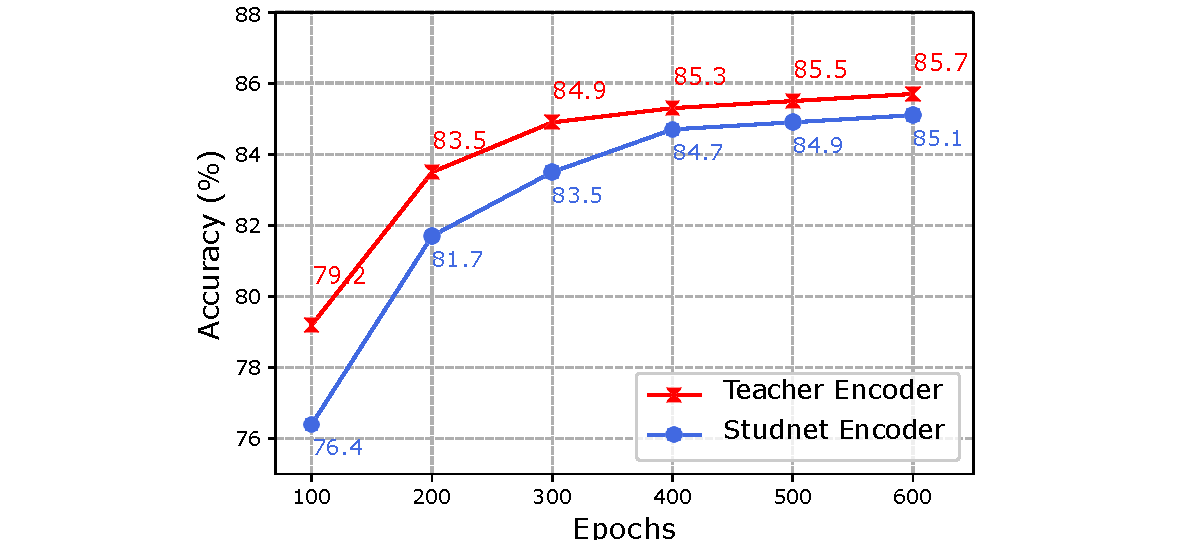
\includegraphics[width=0.95\linewidth]{figures/rebuttal_teacher_student.pdf}
%   \caption{
%     Ablation study on the EMA parameter $\tau_{0}$.
%     The results are reported on the NTU-60 XSub dataset under the
%     linear protocol.
%   }
%   \label{fig:teacher_and_student}
% \end{figure}

\noindent \textbf{Semi-supervised Evaluation:}
In the semi-supervised protocol, we add an MLP head to the pre-trained
encoder and then fine-tune the entire network using only 1\% and 10\% of the training data.
We use the AdamW optimizer with a
weight decay of 0.05. The learning rate starts at 0 and linearly increases to 3e-4
for the first 5 epochs, then decreases to 1e-5 according to a cosine decay schedule.
We train the network for a total of 100 epochs with a batch size of 48.
% In the semi-supervised evaluation protocol, only 1\% and 10\% of the training
% data are employed for fine-tuning, maintaining consistency with other training settings.
Evaluations on the NTU-60 dataset and comparisons with state-of-the-art approaches
such as HYSP \cite{franco2023hyperbolic}, SkeAttnCLR \cite{Hua2023SkeAttnCLR}, and MAMP
\cite{mao2023masked} are conducted.
As depicted in \cref{tab:semi-supervised},
Skeleton2vec demonstrates significant superiority over these methods, particularly
when utilizing only 1\% of the training data. Specifically, on the XSub and XView
settings, Skeleton2vec outperforms MAMP by 9.7\% and 7.5\%, respectively,
affirming the superiority of the proposed Skeleton2vec pretraining framework.

\noindent \textbf{Fine-tuning Evaluation:}
Under the fine-tuning protocol, we employ the same training settings as the
semi-supervised protocol, but fine-tuned using 100\% of the training data.
% In the fine-tuning protocol, we add an MLP head to the pre-trained
% encoder and then fine-tune the entire network. We use the AdamW optimizer with a
% weight decay of 0.05. The learning rate starts at 0 and linearly increases to 3e-4
% for the first 5 epochs, then decreases to 1e-5 according to a cosine decay schedule.
% We train the network for a total of 100 epochs with a batch size of 48.
Evaluation of the fine-tuning results on the NTU-60 and NTU-120 datasets is
presented in \cref{tab:fine-tuning}. Our proposed Skeleton2vec consistently outperforms
previous methods based on the masked prediction task, including SkeletonMAE \cite{yan2023skeletonmae}
and MotionBERT \cite{zhu2023motionbert}, across all datasets.
Additionally, our approach demonstrated comparable or even superior performance compared
to the state-of-the-art method MAMP \cite{mao2023masked} on most datasets, particularly
on the NTU-60 XView dataset. However, the advantage of our method under the
fine-tuning protocol seems less pronounced compared to the semi-supervised protocol.
This is primarily because the model achieves a good fit when fine-tuned using a
sufficient amount of training data (100\%), thus mitigating the performance differences
introduced by various pre-training methods.
This phenomenon is also evident in the results of the semi-supervised protocol (\cref{tab:semi-supervised}),
where the performance improvement from using 10\% of the training data is much smaller
than that from using 1\% of the training data.
% Furthermore, the choice of training settings and tricks can significantly
% impact the results under the fine-tuning protocol.
% Moreover, our
% approach demonstrates comparable results to the current state-of-the-art method,
% MAMP \cite{mao2023masked}, and achieves further improvements on the NTU-60 XView dataset.

\noindent \textbf{Transfer Learning Evaluation:}
In the transfer learning evaluation protocol, pretraining is initially performed
on the source dataset and subsequently fine-tuned on the target dataset. The
source datasets used in our experiments are NTU-60 and NTU-120, with the target
dataset being PKU-MMD II. As illustrated in \cref{tab:transfer}, our proposed
Skeleton2vec surpasses the state-of-the-art method MAMP by 2.4\% and 1.9\% when
using NTU-60 and NTU-120 as source datasets, respectively. This underscores the
robustness of features learned through the Skeleton2vec framework.

\subsection{Ablation Study}
We conducted an extensive ablation study on NTU-60 XSub dataset and NTU-60 XView dataset to analyze the proposed
SKeleton2vec framework. Unless otherwise specified, we pre-train the model for 200
epochs and report the results under the linear evaluation protocol.

\noindent \textbf{Teacher vs. Student:}
Compared to offline pre-training a teacher network using additional labeled data or
pretext tasks to guide a student, our Skeleton2vec employs online updating of the
teacher's parameters through EMA of the student's parameters.
This approach does not require labeled data or additional training stages,
making it a highly cost-effective choice.
To demonstrate the teacher's ability to guide the student through online EMA updates,
we illustrate in \cref{fig:teacher_and_student} the performance evolution of both teacher and student on the
NTU-60 XSub dataset throughout the training process.
It is evident that the teacher consistently outperforms the student,
indicating that the teacher has learned high-level semantics and can effectively guide the student.

\noindent \textbf{Teacher Weight Update:}
We regulate the update frequency of teacher's weights by adjusting the parameter
$\tau_{0}$ in the exponential moving average. In \cref{fig:ema_ablation}, we compared the
impact of four different values of $\tau_{0}$ on the pre-training performance of the model.
It is observed that employing smaller $\tau_{0}$ values (0.99, 0.999) leads to a rapid
performance improvement in the early stages of training (first 100 epochs). However,
as training progresses, the performance growth diminishes, and in some cases,
a decline is observed. Conversely, overly large values of $\tau_{0}$ (0.99999) significantly
slow down the convergence of training, incurring impractical time costs.
Through experimentation, we found that using an appropriate $\tau_{0}$ value (0.9999)
achieves a balanced convergence speed and growth potential,
resulting in optimal performance.

\begin{figure}[tb]
  \begin{minipage}[b]{0.48\linewidth}
    \centering
    \captionof{table}{
      Performance comparison in the transfer learning protocol.
      The source datasets are NTU-60 and NTU-120, and the target dataset is PKU-II.
    }
    \begin{tabular}{l c c}
      \toprule
      \multirow{2}{*}{Method} &
      \multicolumn{2}{c}{To PKU-II} \\
      & NTU 60 & NTU 120 \\
      \midrule
      % LongTGAN \cite{zheng2018unsupervised} & 44.8 & - \\
      % MS2L \cite{lin2020ms2l} & 45.8 & - \\
      ISC \cite{thoker2021skeleton} & 51.1 & 52.3 \\
      CMD \cite{mao2022cmd} & 56.0 & 57.0 \\
      HaLP+CMD \cite{shah2023halp} & 56.6 & 57.3 \\
      SkeletonMAE \cite{wu2023skeletonmae} & 58.4 & 61.0 \\
      MAMP \cite{mao2023masked} & 70.6 & 73.2 \\
      \midrule
      \textbf{Skeleton2vec(Ours)} & \textbf{73.0} & \textbf{75.1} \\
      \bottomrule
    \end{tabular}
    \label{tab:transfer}
  \end{minipage}\hfill
  \begin{minipage}[b]{0.48\linewidth}
    \centering
    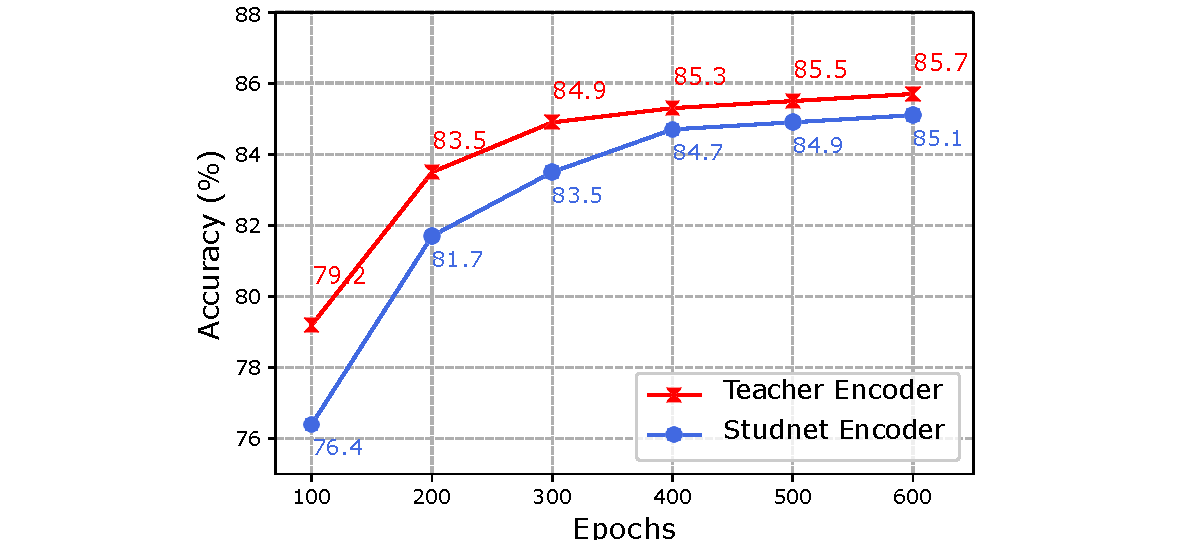
\includegraphics[width=0.80\linewidth]{figures/rebuttal_teacher_student.pdf}
    \caption{
      The performance comparison between teacher and student on the NTU-60 XSub
      dataset across the training process, under the linear protocol.
    }
    \label{fig:teacher_and_student}
  \end{minipage}
  \vspace{-15pt}
\end{figure}

\begin{figure}[tb]
  \begin{minipage}[b]{0.48\linewidth}
    \centering
    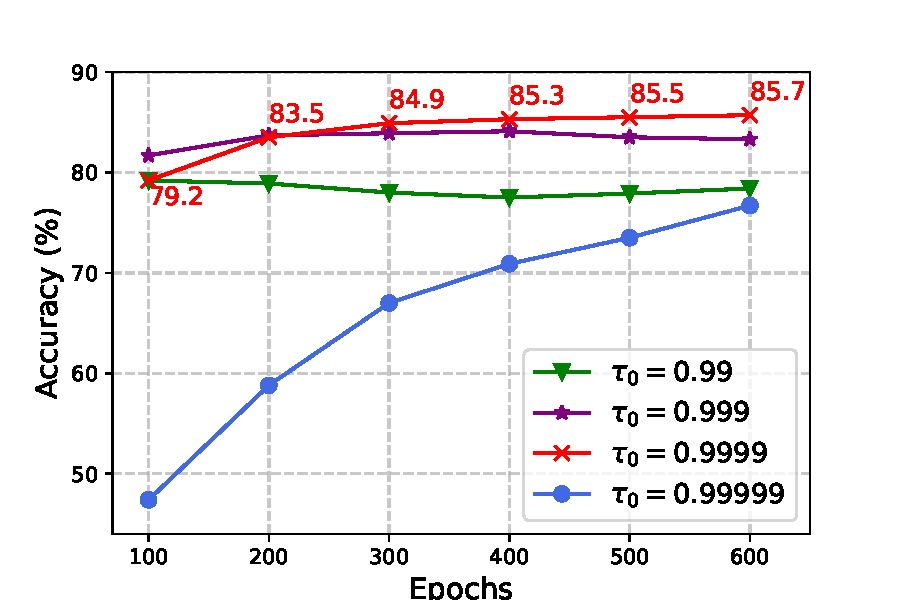
\includegraphics[width=0.75\linewidth]{figures/ema_ablation.pdf}
    \caption{
      Ablation study of EMA parameter $\tau_{0}$ on the NTU-60 XSub dataset
      under linear protocol.
      % Ablation study on the EMA parameter $\tau_{0}$.
      % The results are reported on the NTU-60 XSub dataset under the linear protocol.
      }
    \label{fig:ema_ablation}
  \end{minipage}
  \hfill
  \begin{minipage}[b]{0.48\linewidth}
    \centering
    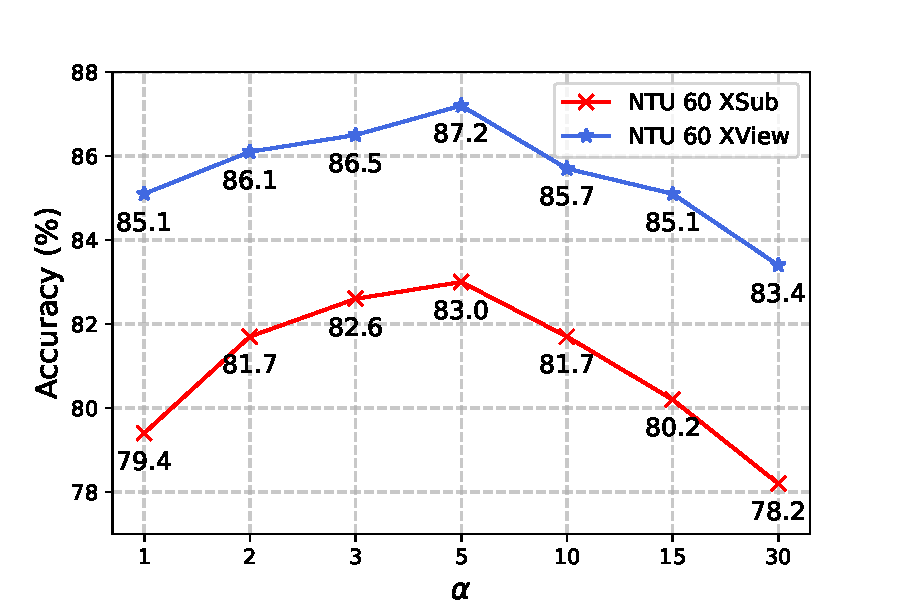
\includegraphics[width=0.75\linewidth]{figures/alpha_ablation.pdf}
    \caption{
      Ablation study of the tube length $\alpha$ on the NTU-60 XSub and XView datasets.
      % Ablation study on the tube length $\alpha$.
      % $\alpha=0$ is equivalent to random masking, while $\alpha=30$, which is the length of the input sequence, is equivalent to single-tube masking.
      }
    \label{fig:alpha_ablation}
  \end{minipage}
  \vspace{-14pt}
\end{figure}

\begin{figure}[tb] \scriptsize
    \captionof{table}{Ablation study on the \textbf{Motion-Aware Multi-Tube (MAMT)} masking strategy. $\alpha$ represents the length of each tube, while $\beta$ denotes the parameter of motion-aware sampling. $m$ denotes the masking ratio.}
    \centering
    \begin{subfigure}[t]{0.5\linewidth}
        \centering
        \begin{tabular}{c c c c c}
            \toprule
            \multirow{2}{*}{Strategy} & \multirow{2}{*}{$\alpha$} & \multirow{2}{*}{$\beta$} & \multicolumn{2}{c}{NTU 60} \\
            & & & XSub & XView \\
            \midrule
            Random & 1 & 0.0 & 79.4 & 85.1 \\
            Single-tube & 30 & 0.0 & 78.2 & 83.4 \\
            Multi-tube & 5 & 0.0 & 83.0 & 87.2 \\
            \textbf{MAMT(Ours)} & 5 & 0.1 & \textbf{83.5} & \textbf{87.7} \\
            \bottomrule
        \end{tabular}
        \caption{Masking strategy.}
        \label{tab:masking_strategy}
    \end{subfigure}
    \hfill
    \begin{subfigure}[t]{0.24\linewidth}
        \centering
        \begin{tabular}{c c c}
            \toprule
            \multirow{2}{*}{$\beta$} & \multicolumn{2}{c}{NTU 60} \\
            & XSub & XView \\
            \midrule
            0.0 & 83.0 & 87.2 \\
            0.1 & \textbf{83.5} & \textbf{87.7} \\
            0.2 & 82.1 & 87.0 \\
            0.3 & 79.5 & 86.3 \\
            \bottomrule
        \end{tabular}
        \caption{Motion-aware sampling}
        \label{tab:beta}
    \end{subfigure}
    \hfill
    \begin{subfigure}[t]{0.24\linewidth}
        \centering
        \begin{tabular}{c c c}
            \toprule
            \multirow{2}{*}{$m$} & \multicolumn{2}{c}{NTU 60} \\
            & XSub & XView \\
            \midrule
            0.80 & 83.1 & 86.7 \\
            0.85 & 83.3 & 87.3 \\
            0.90 & \textbf{83.5} & \textbf{87.7} \\
            0.95 & 77.1 & 82.1 \\
            \bottomrule
        \end{tabular}
        \caption{Masking ratio}
        \label{tab:masking_ratio}
    \end{subfigure}
    \label{tab:masking_ratio_and_beta}
    \vspace{-18pt}
\end{figure}

\noindent \textbf{Masking Strategy:}
% \cref{tab:masking_strategy} illustrates the effectiveness of our proposed
% Motion-Aware Multi-Tube (MAMT) masking strategy.
% We compared its performance with other masking strategies.
% We compared its performance with random masking
% and tube masking (without motion-aware sampling).
% The results indicate a significant
% performance boost with multi-tube masking compared to random and single-tube masking, showing improvements
% of 3.6\% and 2.1\% under the XSub and XView testing protocols of the NTU-60 dataset,
% respectively. This underscores the capability of tube segmentation to compel the
% model into effective long-range motion modeling.
\cref{tab:masking_strategy} presents a performance comparison between our
proposed Motion-Aware Multi-Tube (MAMT) masking strategy and other methods.
It is evident that compared to random masking and single-tube masking,
multi-tube masking yields a significant performance improvement,
validating the effectiveness of dividing into multiple tubes.
We visually illustrate the differences between the three masking strategies
in \cref{fig:masking_cmp}. It can be observed that random masking samples a different
masking map for each frame, single-tube masking shares a single masking map
across all frames, while multi-tube masking is a compromise between the two,
sharing the masking map only among several adjacent frames.
This approach mitigates information leakage while encouraging the model to
establish long-range spatiotemporal relationships.
Moreover, motion-aware sampling
further improves performance, highlighting the value of guiding the model to focus
on semantically rich action regions. A detailed analysis of hyperparameters in
MAMT masking will be presented in subsequent sections.

\begin{figure}[tb]
    \centering
    \begin{minipage}[b]{0.48\linewidth}
        \centering
        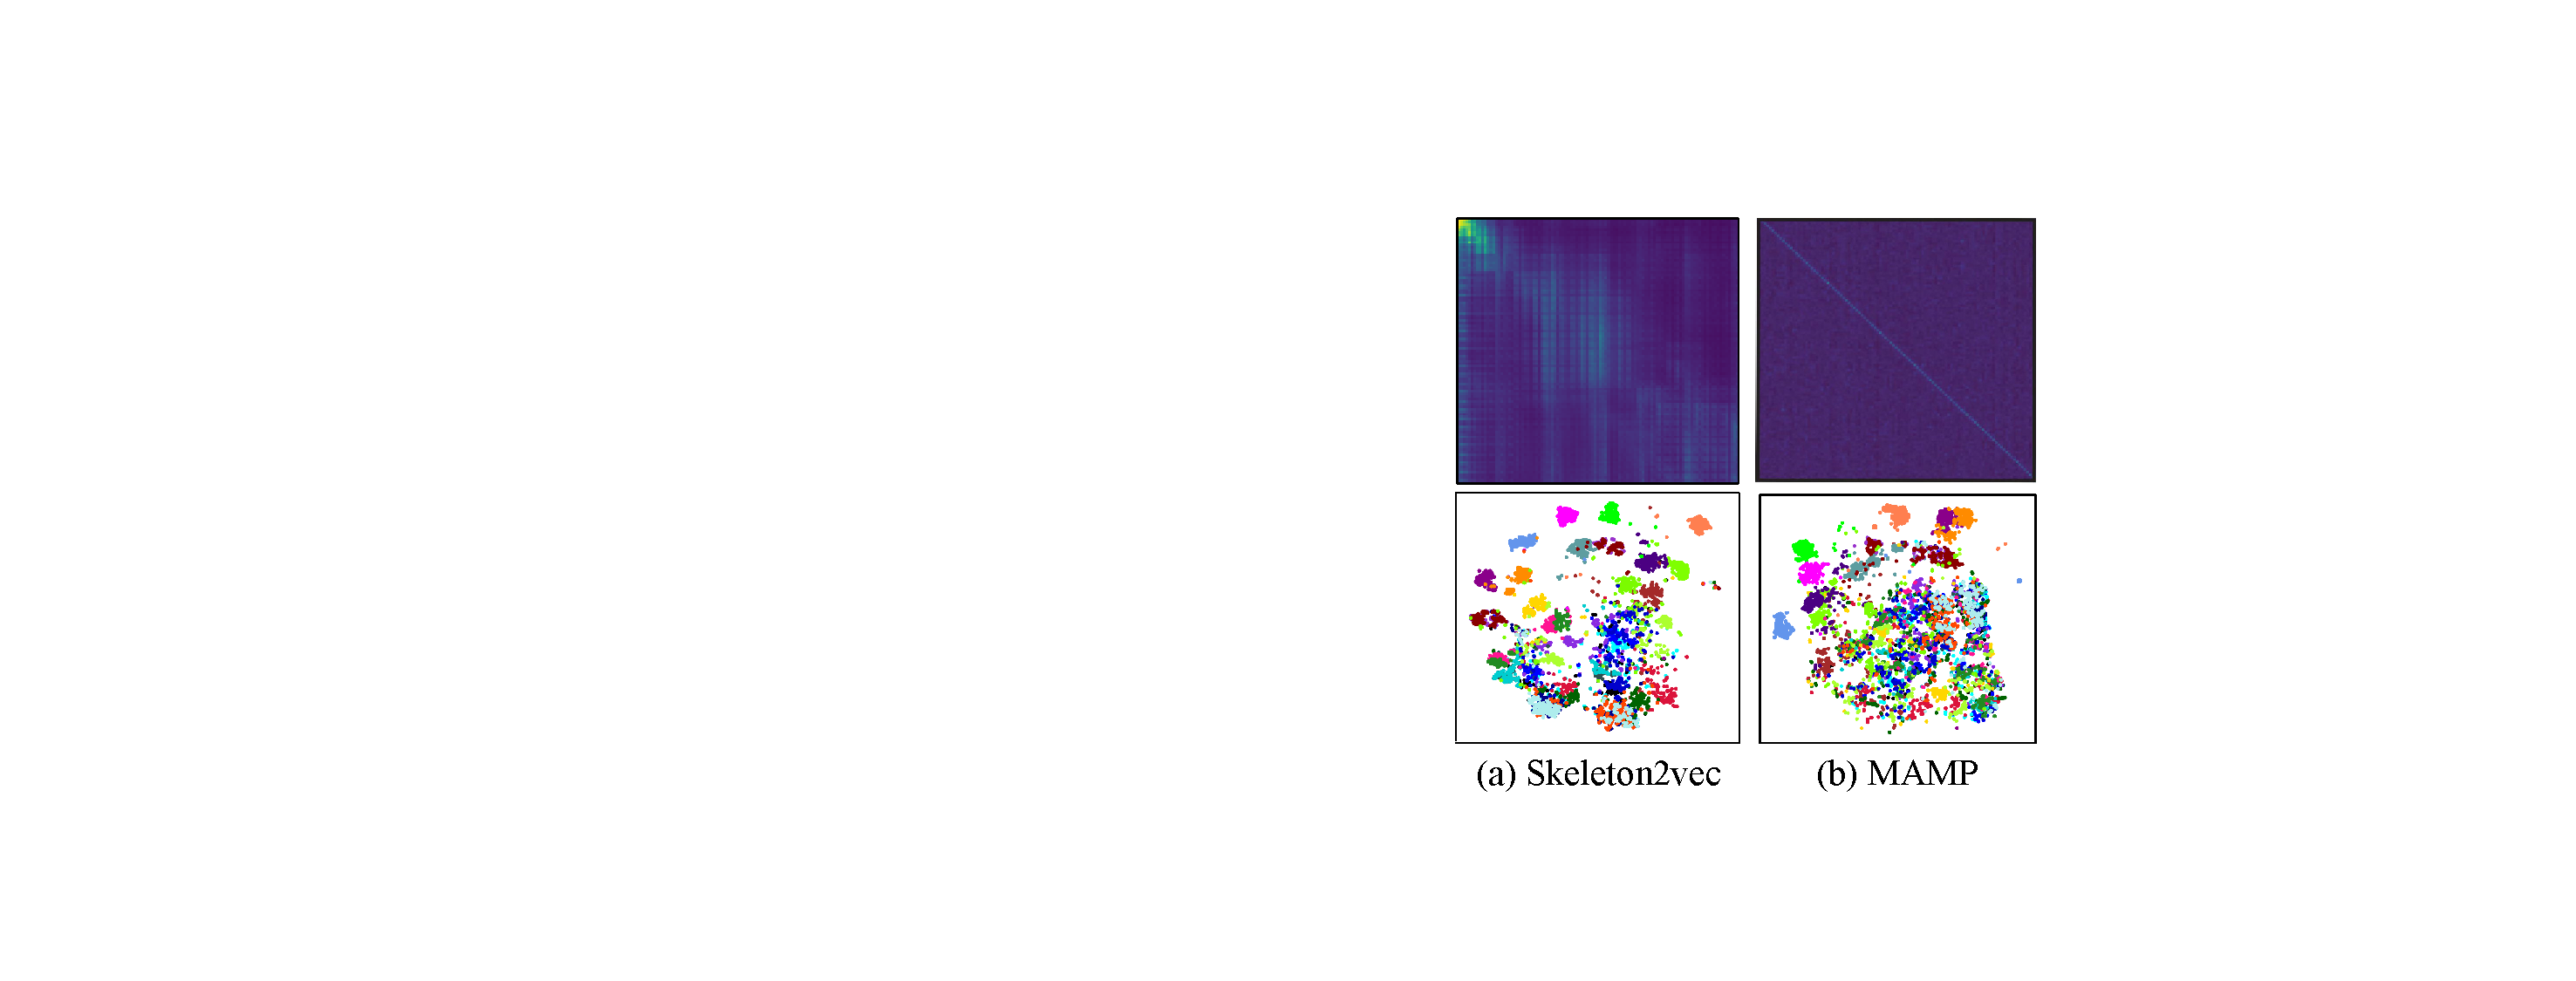
\includegraphics[width=0.70\linewidth]{figures/fig_qualitative.pdf}
        \caption{
          Visualization of the average multi-head self-attention matrices(Top) and
          t-SNE feature embeddings for 30 classes in the NTU60-XSub dataset(Bottom).
        }
        \label{fig:qualitative}
    \end{minipage}\hfill
    \begin{minipage}[b]{0.49\linewidth}
        \centering
        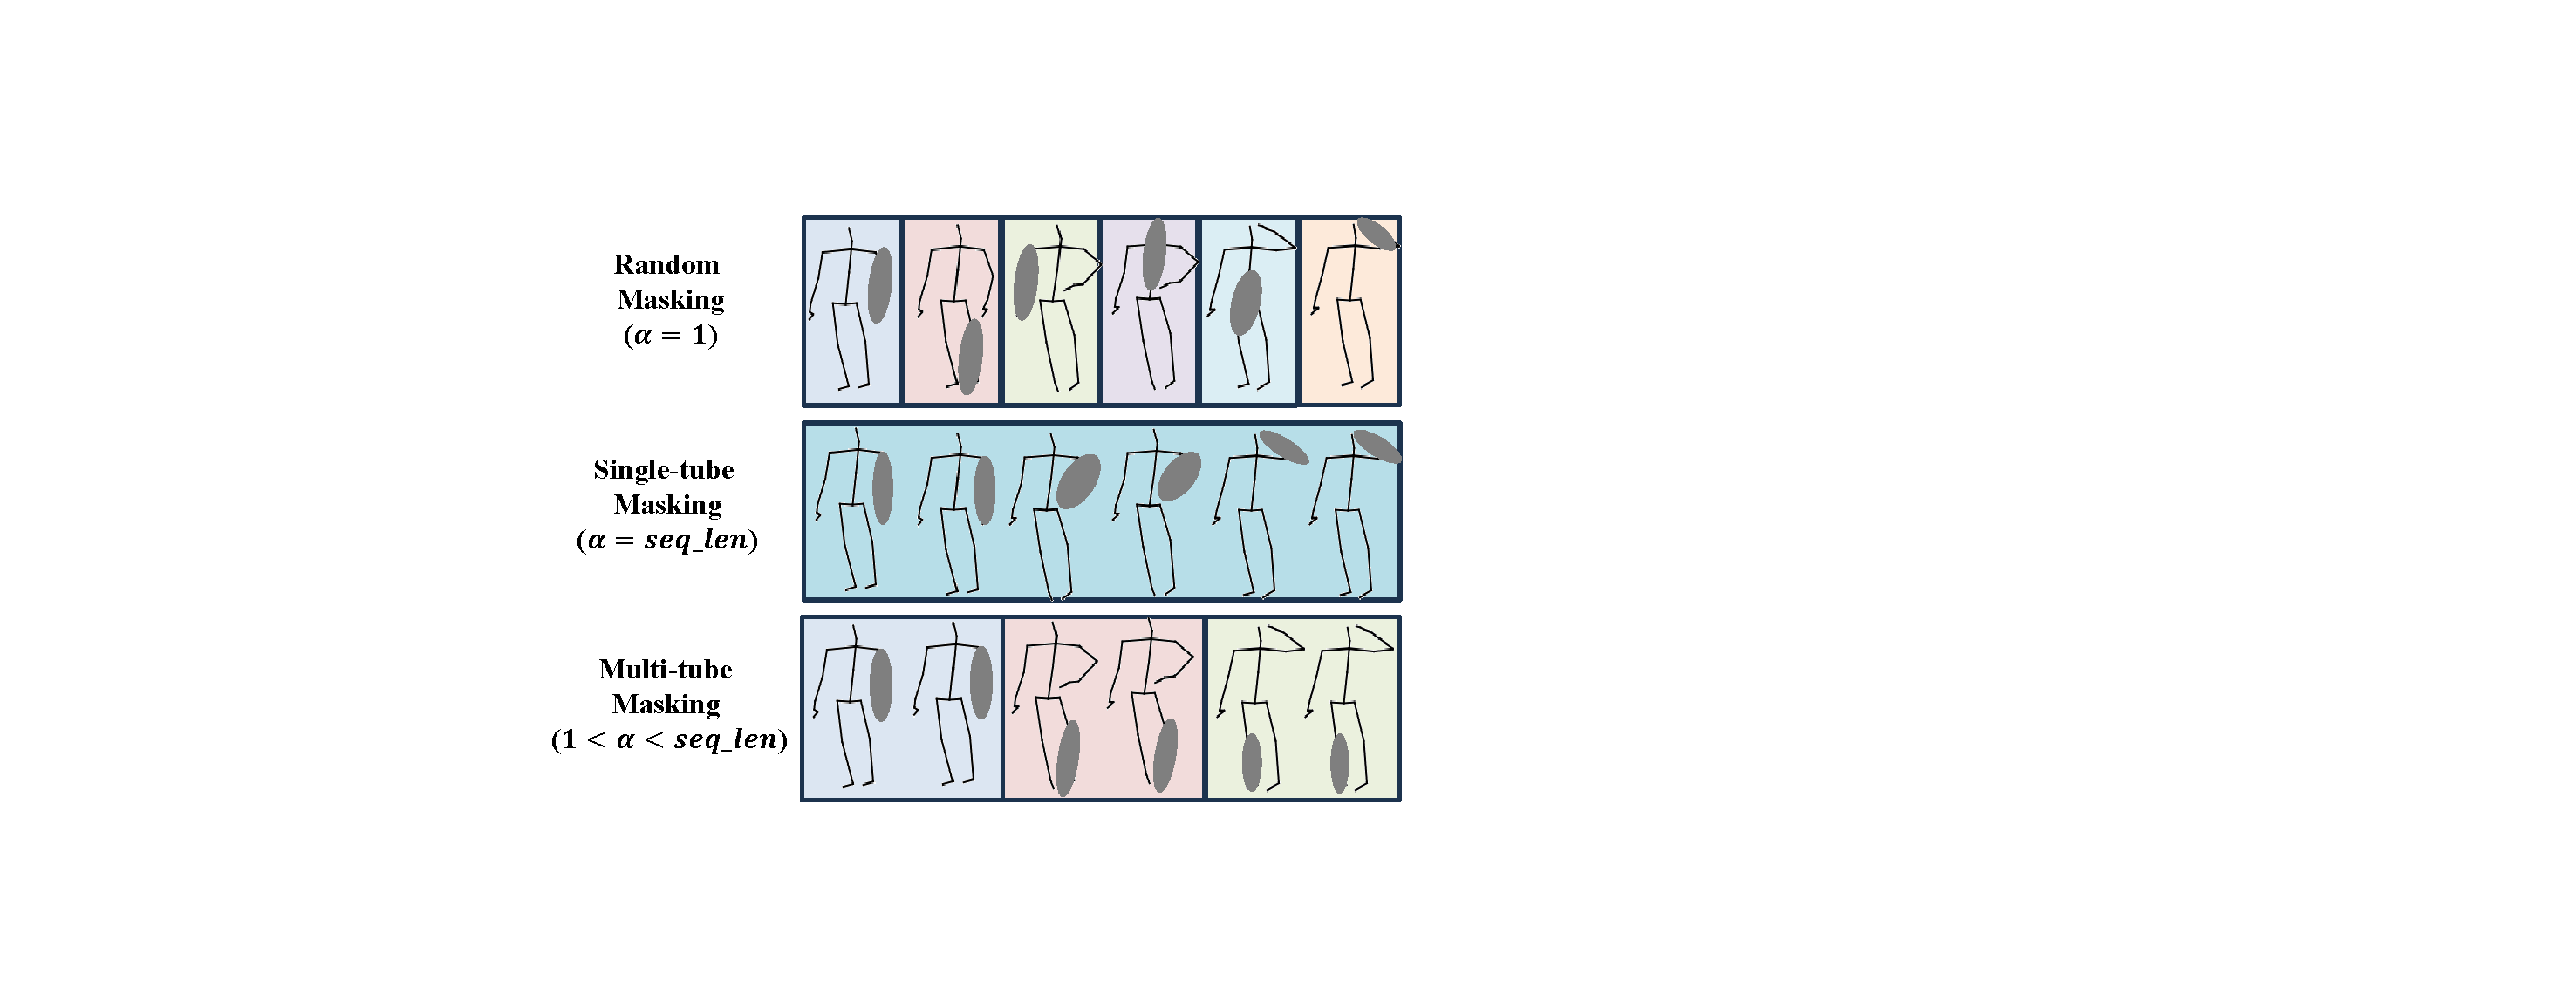
\includegraphics[width=0.90\linewidth]{figures/fig_masking_cmp.pdf}
        \caption{
          Intuitive comparison of different masking strategies.
          $\alpha$ represents the tube length, and $seq_len$ represents the sequence length.
        }
        \label{fig:masking_cmp}
    \end{minipage}
    \vspace{-15pt}
\end{figure}

\noindent \textbf{Tube Length:}
We investigated the impact of the length $\alpha$ of each tube on pre-training performance.
As depicted in \cref{fig:alpha_ablation}, excessively short tube lengths result
in information leakage between adjacent frames, leading to a performance decline.
On the other hand, overly long tube lengths pose excessively challenging pre-training
tasks, impairing the model's learning capacity, as discussed in \cref{sec:motion-aware_tube_masking}.
Hence, selecting an appropriate tube length is crucial. Considering the results
from \cref{fig:alpha_ablation}, we identified a tube length of $\alpha=5$ as
optimal, achieving the best balance and performance.

\noindent \textbf{Motion-aware Sampling:}
We compared the performance of learned representations under different motion-aware
sampling parameters $\beta$. As shown in \cref{tab:beta}, selecting an appropriate
sampling parameter enhances pre-training performance compared to not using
motion prior information ($\beta=0$). However, excessively large sampling parameters
can result in overly fixed sampling of joints, leading to a loss of diversity and
a subsequent performance decline. We empirically found that a sampling parameter of
$\beta=0.1$ yields the best results.

\noindent \textbf{Masking Ratio:}
In \cref{tab:masking_ratio}, we compared the influence of different masking ratios
on the results. It is evident that excessively large or small masking ratios can
impair the final performance. We ultimately selected a masking ratio of 90\% to
achieve optimal results.

\noindent \textbf{Qualitative Results:}
% To demonstrate the superiority of using contextualized representations
% as self-supervised prediction targets in our Skeleton2vec,
% We compared the average multi-head self-attention matrices and the output
% feature embeddings of the last layer of the pre-trained encoders for
% Skeleton2vec and MAMP \cite{mao2023masked}. The visualization results are
% depicted in \cref{fig:qualitative}, where the feature embeddings are
% derived from samples of 30 classes selected from the NTU-60 XSub test set
% and dimensionality reduction is performed using t-SNE.
% It is observed that compared to MAMP \cite{mao2023masked},
% Skeleton2vec exhibits a more uniform and global attention distribution,
% primarily attributed to the utilization of globally contextualized representations
% as prediction targets rather than merely local motion context.
% Additionally, the features outputted by our Skeleton2vec demonstrate
% significantly better separability, affirming the effectiveness of our approach.
To illustrate the effectiveness of contextualized representations as self-supervised targets
in Skeleton2vec, we compared the average multi-head self-attention matrices and
output feature embeddings of pre-trained encoders between Skeleton2vec and MAMP \cite{mao2023masked}.
Visualization results (see \cref{fig:qualitative}) depict feature embeddings from a subset
of 30 classes from the NTU-60 XSub test set, with dimensionality reduction via t-SNE.
Compared to MAMP, Skeleton2vec shows a more uniform and global attention distribution,
thanks to its use of globally contextualized representations as prediction targets
rather than local motion context alone. Furthermore, Skeleton2vec's feature outputs exhibit
significantly improved separability, confirming the efficacy of our approach.
\vspace{-5pt}
\section{Conclusion}
\vspace{-5pt}
In this work, we propose Skeleton2vec, a novel self-supervised learning framework
for 3D skeleton-based action recognition. We demonstrated the superiority of utilizing
global contextualized representations built by a teacher model as the prediction target
for the masked prediction task, compared to isolated raw joints or temporal motion with
local context. Furthermore, considering the high spatiotemporal correlation in skeleton
sequences, we proposed the motion-aware multi-tube masking strategy to compel the model into
effective long-range motion modeling. Extensive experiments conducted on three large-scale
prevalent benchmarks validated the effectiveness of our approach. The experimental results
showcased outstanding performance of our proposed Skeleton2vec,
achieving state-of-the-art results across multiple testing protocols.


% \clearpage\mbox{}Page \thepage\ of the manuscript.
% \clearpage\mbox{}Page \thepage\ of the manuscript.
% \clearpage\mbox{}Page \thepage\ of the manuscript.
% \clearpage\mbox{}Page \thepage\ of the manuscript.
% \clearpage\mbox{}Page \thepage\ of the manuscript. This is the last page.
\par\vfill\par
% Now we have reached the maximum length of an ECCV \ECCVyear{} submission (excluding references).
% References should start immediately after the main text, but can continue past p.\ 14 if needed.
% \clearpage  % TODO REVIEW/FINAL: This \clearpage needs to be removed from both review and camera-ready versions.


% ---- Bibliography ----
%
% BibTeX users should specify bibliography style 'splncs04'.
% References will then be sorted and formatted in the correct style.
%
\bibliographystyle{splncs04}
\bibliography{main}
\end{document}
